% ============================================================================
% AI-Driven Crop Yield Prediction System — Final Dissertation
% Kuzey Erturk, F330035
% Loughborough University, Computer Science
% ============================================================================

\documentclass[12pt,a4paper]{report}

% --- Packages ---
\usepackage[utf8]{inputenc}
\usepackage[T1]{fontenc}
\usepackage{graphicx}
\usepackage{booktabs}
\usepackage{amsmath,amssymb}
\usepackage{hyperref}
\usepackage{geometry}
\usepackage{setspace}
\usepackage{caption}
\usepackage{subcaption}
\usepackage{float}
\usepackage{multirow}
\usepackage{array}
\usepackage{longtable}
\usepackage{enumitem}
\usepackage{xcolor}
\usepackage{listings}
\usepackage[numbers]{natbib}
\usepackage{pdflscape}
\usepackage{tabularx}

\geometry{margin=2.5cm}
\onehalfspacing
\graphicspath{{reportimages/}}

\hypersetup{
    colorlinks=true,
    linkcolor=black,
    citecolor=blue,
    urlcolor=blue,
}

% --- Custom commands ---
\newcommand{\rsq}{R\textsuperscript{2}}
\newcommand{\degrees}{$^{\circ}$C}
\newcommand{\tha}{t\,ha\textsuperscript{$-1$}}

% ============================================================================
\begin{document}

% --- Title Page ---
\begin{titlepage}
\centering
\vspace*{2cm}
{\LARGE\bfseries AI-Driven Crop Yield Prediction System\par}
\vspace{1.5cm}
{\Large Dissertation \par}
\vspace{1cm}
{\large Kuzey Erturk\\
Student ID: F330035\par}
\vspace{1cm}
{\large Supervisor: Prof.\ Nina Dethlefs\par}
\vspace{1cm}
{\large Department of Computer Science\\
Loughborough University\par}
\vspace{1cm}
{\large April 2026\par}
\vfill
\end{titlepage}

% --- Abstract ---
\begin{abstract}
Accurate crop yield prediction is essential for food security planning and agricultural decision-making, yet data scarcity limits model performance in regions such as the United Kingdom, where only four administrative regions report annual yields. This project develops and evaluates machine learning models for predicting UK crop yields (wheat, winter barley, spring barley, oats, and oilseed rape) using 47 engineered weather features aligned with crop phenology. Initial UK-only models achieved moderate performance (\rsq{} = 0.15--0.50), constrained by small sample sizes (52 observations per crop).

To address this, a cross-country data augmentation strategy was developed, pooling yield and weather data from France, Germany, Ireland, the Netherlands, Belgium, and Denmark. Direct pooling of raw data failed due to differing yield levels and climate baselines between countries. A \textbf{detrended anomaly transfer} methodology was developed: yields are detrended per region to isolate weather-driven anomalies, and weather features are standardised to per-region z-scores, removing climate baseline differences. This enables meaningful cross-country pooling.

The pooled anomaly approach substantially improved prediction accuracy: wheat \rsq{} increased from 0.28 to 0.70, spring barley from 0.22 to 0.76, and oats from $-0.46$ to 0.48. A rescaled direct transfer experiment demonstrated that weather--yield response curves learned from French data alone can predict UK yield anomalies with positive \rsq{} (0.14--0.65) after linear calibration, confirming the transferability of these relationships. An investigation into scenario-adaptive source country selection found no improvement over static pooling, confirming that anomalisation already removes the climate differences that adaptive methods attempt to address. The final models were deployed in an interactive Flask web application for real-time yield prediction.
\end{abstract}

% --- Table of Contents ---
\tableofcontents
\listoffigures
\listoftables

% ============================================================================
% CHAPTER 1: INTRODUCTION
% ============================================================================
\chapter{Introduction}

\section{Background and Motivation}

Agricultural productivity faces increasing challenges from climate change, climate variability, and environmental uncertainty. The growing global population,projected to reach 9.7 billion by 2050 \citep{un2019}, and rising food demand necessitate efficient farming practices to manage limited natural resources sustainably. Climate change has intensified extreme weather events such as droughts, floods, and unseasonal temperatures, creating greater uncertainty in crop production cycles \citep{ipcc2021}. Accurate yield prediction tools are essential to mitigating these uncertainties, enabling proactive planning rather than reactive response.

In the UK, agriculture contributes approximately \pounds10 billion annually to the economy, with cereals and oilseed crops, principally wheat, barley, oats, and oilseed rape in which they cover over 3 million hectares of farmland \citep{defra2023}. Wheat alone accounts for approximately 1.8 million hectares, producing around 14 million tonnes annually \citep{ahdb2023a}. Weather variability significantly impacts yields, for example the wet summer of 2012 caused wheat yields to drop nearly 19\% below average, from 7.8~\tha{} to 6.3~\tha{} \citep{defra2012}. This clearly demonstrates how vulnerable UK agriculture is to climatic extremes.

Accurate crop yield prediction enables farmers to optimise resource allocation, plan harvests, and mitigate financial risks. Traditional forecasting methods rely on simple statistical approaches or farmer intuition, which often fail to capture the complex, non-linear interactions between environmental factors and crop performance \citep{vanklompenburg2020}. Machine learning offers the potential to model these relationships by learning from historical patterns in weather and yield data, with studies showing improvements of 10--30\% over traditional regression methods \citep{chlingaryan2018}.

However, a fundamental challenge for UK crop yield prediction is \textbf{data scarcity}. With only four administrative regions (England, Wales, Scotland, Northern Ireland) reporting annual yields over approximately 20~years, each crop has fewer than 84~data points for training which is below the usual recommendations of most machine learning approaches \citep{corcoran2023}. This project addresses this challenge by developing a cross-country data augmentation strategy that pools yield--weather data from climatically similar European countries, effectively multiplying the available training data.

\section{Research Questions and Objectives}

This project addresses three research questions:

\begin{enumerate}
    \item \textbf{RQ1:} Can machine learning models predict UK crop yields from weather data alone, and which weather features are most important for each crop?
    \item \textbf{RQ2:} Can data pooling from climatically similar European countries improve UK crop yield predictions, and under what conditions does transfer succeed or fail?
    \item \textbf{RQ3:} Are weather--yield response curves transferable between countries, and can models trained on foreign data predict UK yields?
\end{enumerate}

The corresponding objectives are:

\begin{enumerate}
    \item Compile and integrate multi-source agricultural datasets covering UK yield data (DEFRA), UK weather data (Met Office), European yield data (Eurostat), and European weather data (E-OBS gridded observations).
    \item Engineer weather features capturing seasonal patterns aligned with crop growth stages.
    \item Develop and compare machine learning models including Ridge regression, Random Forest, and SVR for five UK crops.
    \item Implement a cross-country data pooling pipeline including seven European countries.
    \item Develop and evaluate a detrended anomaly transfer methodology that enables meaningful cross-country yield data combination.
    \item Investigate whether scenario-adaptive source country selection can improve upon static pooling.
    \item Deploy the best models in an interactive web application demonstrating practical applicability.
\end{enumerate}

\section{Project Scope}

This project focuses on five major UK crops: wheat, winter barley, spring barley, oats, and oilseed rape (OSR). The UK analysis covers the period 2004--2024 using regional yield data from DEFRA \citep{defra2024} and weather data from the UK Met Office \citep{metoffice2024}. Cross-country data spans 2004--2018 (the common overlap period) across seven countries, though French data goes back to 1995: UK, France, Germany, Ireland, the Netherlands, Belgium, and Denmark. The prediction models use weather-based features only, excluding economic factors (e.g., fertiliser prices) and detailed soil data due to data availability constraints.

\section{Report Structure}

Chapter~2 reviews the relevant literature on crop yield prediction, weather--yield relationships, and cross-country transfer learning. Chapter~3 presents the data sources, feature engineering pipeline, and the three-phase methodology (UK-only models, cross-country pooling, and detrended anomaly transfer). Chapter~4 reports the results across all experimental phases. Chapter~5 discusses the key findings, their implications, and limitations. Chapter~6 concludes and identifies future work directions.


% ============================================================================
% CHAPTER 2: LITERATURE REVIEW
% ============================================================================
\chapter{Literature Review}

\section{Crop Yield Prediction Methods}

Driven by the increasing climate uncertainty globally, the field of crop yield prediction has evolved rapidly; what were once simple statistical calculations have been replaced by advanced computational models capable of capturing the complex, non-linear interactions of modern agriculture. \citet{vanklompenburg2020} conducted a systematic review of 50~studies using ML for crop yield prediction, identifying Random Forest, neural networks, and support vector machines as the most commonly used algorithms. They found that most studies report improvements over traditional regression baselines, but noted that many studies use large-scale national or continental datasets.

\citet{paudel2021} evaluated ML methods (Ridge, KNN, SVR, GBDT) for crop yield forecasting across European countries, achieving a median normalised RMSE of 16.57\%. Their approach pooled subnational regions within each country, having a huge influence on the rationale underlying our cross-country pooling, but applied at a different geographic scale. They acknowledged that model performance degrades for extreme weather years, a challenge we address through our anomaly-based approach.

\citet{jeong2016} demonstrated that Random Forest models can effectively predict global crop yields using gridded climate data, achieving \rsq{} values of 0.51--0.75 for wheat. Their work established Random Forest as a strong baseline for tabular agricultural data, motivating our initial model selection.

\section{Weather--Yield Relationships in European Agriculture}

Understanding which weather variables drive yield variation is central to prediction modelling. \citet{gammans2017} used 65~years of French department-level yield data with panel regression, finding that temperatures above 32\degrees{} reduce wheat yields by 2.9\% per day and that spring barley is the most heat-sensitive cereal ($-4.6$\% at 32\degrees{}+). They identified optimal precipitation at 200--236\,mm during the spring--summer growing season. Crucially, they used the same E-OBS gridded weather data and French departmental structure as our study, providing direct methodological precedent.

\citet{moore2015} conducted the first formal attribution of long-term yield trends to climate change in European agriculture, using data across 349~subnational regions in 11~countries including the UK. They detected a statistically significant ``climate fingerprint'' on all four crops studied: wheat yields were 2.5\% lower and barley 3.8\% lower than they would have been without post-1989 warming. Their method of using detrended data to isolate anomalies caused by weather, while accounting for country-level differences, is relatively similar to the detrending and country-indicator approach we developed in the latter stages of this project.

\citet{zhu2021} applied Random Forest with SHAP (SHapley Additive exPlanations) analysis to attribute European wheat yield shocks across 1,435~subnational units, finding that heat stress has become the primary driver of yield loss in the 2000--2018 period (superseding water stress, which dominated 1980--1999). Their use of SHAP for interpretable feature importance motivates our own SHAP analysis.

\citet{challinor2014} conducted a meta-analysis of 1,700+ crop yield simulations under climate change, finding a temperature coefficient of $-4.9$\% per \degrees{} of warming, with adaptation measures providing a +7.16\% benefit. This provides useful context for interpreting the magnitude of weather effects in our models.

\section{Cross-Country Transfer and Data Augmentation}

A critical challenge in regional crop yield prediction is data scarcity. \citet{corcoran2023} explicitly identified data bottlenecks for UK crop yield analysis, specifically noting the lack of openly accessible crop management and crop plant data across the UK, particularly for non-wheat crops. This directly motivates our cross-country pooling approach as a data augmentation strategy.

The scientific justification for pooling data across European countries rests on the concept of climate similarities. \citet{pugh2016} used climate analogue matching to assess future crop productivity, finding that suitable growing areas shift geographically under climate change rather than disappearing entirely. We extend this concept from descriptive analysis to predictive data augmentation.

Most critically, \citet{ceglar2019} demonstrated that agro-climate zones in Europe are migrating northward at 70--100~km per decade, with the southern maritime zone (currently characterising France) projected to replace the northern maritime zone (currently characterising the UK) under 2\degrees{} of warming. This provides a direct scientific basis for pooling French and UK crop data: France's current weather--yield patterns preview the UK's near-future conditions.

\citet{ronchetti2024} developed a harmonised dataset of 344,282~subnational crop statistics across 27~EU countries, demonstrating the feasibility and value of cross-country agricultural data integration. Their work shows that our manual pipeline for 7~countries could, in principle, be extended to continental scale.

\citet{riedesel2024} studied site-specific heat and drought impacts on German wheat, finding that site conditions cause 2--3$\times$ variation in stress-related yield losses. This helps explain why German data transfers poorly to UK conditions. The continental climate introduces response differences that cannot be overcome by simple pooling.

\section{Transfer Learning and Domain Adaptation}

The concept of training on one domain and predicting in another is well-established in machine learning as transfer learning or domain adaptation \citep{pan2010}. In agricultural contexts, this manifests as training on data-rich countries and predicting in data-poor ones. However, direct transfer faces fundamental challenges: different cultivars, soil types, farming practices, and climate baselines between countries mean that a model trained on absolute yields from one country will probably mispredict another.

\citet{dinh2022} addressed the methodological challenge of model validation with small datasets, proposing Leave-Two-Out cross-validation as a more robust alternative to Leave-One-Out for sample sizes below 100. Their work validates our use of LOOCV while cautioning about its tendency to favour model complexity which is a concern we address through Ridge regularisation.

\citet{evans2025} provided a critical perspective on space-for-time substitution (SFTS). It is the assumption that spatial variation in climate can substitute for temporal variation. They warned that SFTS can be ``misleading in magnitude and direction'' due to acclimation effects at different timescales. Our cross-country pooling is fundamentally a form of SFTS, and our negative direct transfer results are consistent with their concerns. However, our anomaly-based approach mitigates this by transferring the \emph{direction and relative pattern} of weather–yield responses (e.g., that above-normal 
  summer temperatures reduce yields) rather than absolute predictions of yield levels.

\section{Gap Analysis}

The literature reveals several gaps that this project addresses:

\begin{enumerate}                                                                                                                                                  
      \item \textbf{UK-specific data scarcity:} Most European crop yield studies use countries with hundreds of subnational regions (France: 96~departments, Germany:
   16~states). The UK's four administrative regions create a severe data constraint that limits ML model performance, as identified by \citet{corcoran2023}, yet no  
  study has attempted to resolve this through cross-country data augmentation.                                                                                       
      \item \textbf{Cross-country pooling for yield prediction:} While subnational pooling within individual countries is established \citep{paudel2021}, pooling    
  yield data \emph{across} countries for crop yield prediction has not been systematically explored. The conditions under which such transfer succeeds or fails, and
   which countries make suitable data partners remain uncharacterised.
      \item \textbf{Anomaly-based transfer methodology:} Yield detrending and weather z-score standardisation are individually well-established techniques, but their
   combination as a strategy to enable cross-country data pooling has not been evaluated. This project proposes and tests this combination as a principled approach  
  to removing the country-specific differences (yield levels, climate baselines) that cause na\"{\i}ve pooling to fail.
      \item \textbf{Adaptive vs.\ static source selection:} Given that different countries have different climates, whether dynamically selecting source countries   
  based on weather scenario similarity can improve upon static pooling has not been investigated.                                                                    
  \end{enumerate}


% ============================================================================
% CHAPTER 3: DATA AND METHODOLOGY
% ============================================================================
\chapter{Data and Methodology}

This chapter describes the data sources, feature engineering pipeline, and the three-phase modelling approach used to progressively improve UK crop yield predictions: (1)~UK-only baseline models, (2)~cross-country data collection and initial pooling experiments, and (3)~the detrended domain adaptation approach.

% --------------------------------------------------
\section{UK Data Sources}
% --------------------------------------------------

\subsection{Yield Data}

Crop yield data was obtained from the UK Government's official cereal and oilseed production statistics \citep{defra2024}. The dataset provides annual yield figures (\tha{}) and harvested area (hectares) for major crops across four UK regions.

\begin{table}[H]
\centering
\caption{UK yield data source summary}
\label{tab:uk_yield_source}
\begin{tabular}{ll}
\toprule
\textbf{Attribute} & \textbf{Details} \\
\midrule
Source & GOV.UK Cereal and Oilseed Rape Production Statistics \\
Time period & 2004--2024 (21~years) \\
Regions & England, Wales, Scotland, Northern Ireland \\
Crops & Wheat, Winter Barley, Spring Barley, Oats, OSR \\
Variables & Yield (\tha{}), Area (hectares) \\
\bottomrule
\end{tabular}
\end{table}

\subsection{Weather Data}

Monthly weather data was obtained from the UK Met Office regional climate series \citep{metoffice2024}, providing monthly averages for each UK region.

\begin{table}[H]
\centering
\caption{UK weather data source summary}
\label{tab:uk_weather_source}
\begin{tabular}{ll}
\toprule
\textbf{Attribute} & \textbf{Details} \\
\midrule
Source & UK Met Office Regional Climate Series \\
Time period & 2004--2024 (monthly records) \\
Regions & England, Wales, Scotland, Northern Ireland \\
Variables & Tmax (\degrees{}), Tmin (\degrees{}), Rainfall (mm), Sunshine (hrs), Frost (days) \\
\bottomrule
\end{tabular}
\end{table}

Figure~\ref{fig:uk_yields_overview} shows the yield time series for all crops and regions, highlighting inter-annual variability and notable events such as the 2012 wet summer.

\begin{figure}[H]
\centering
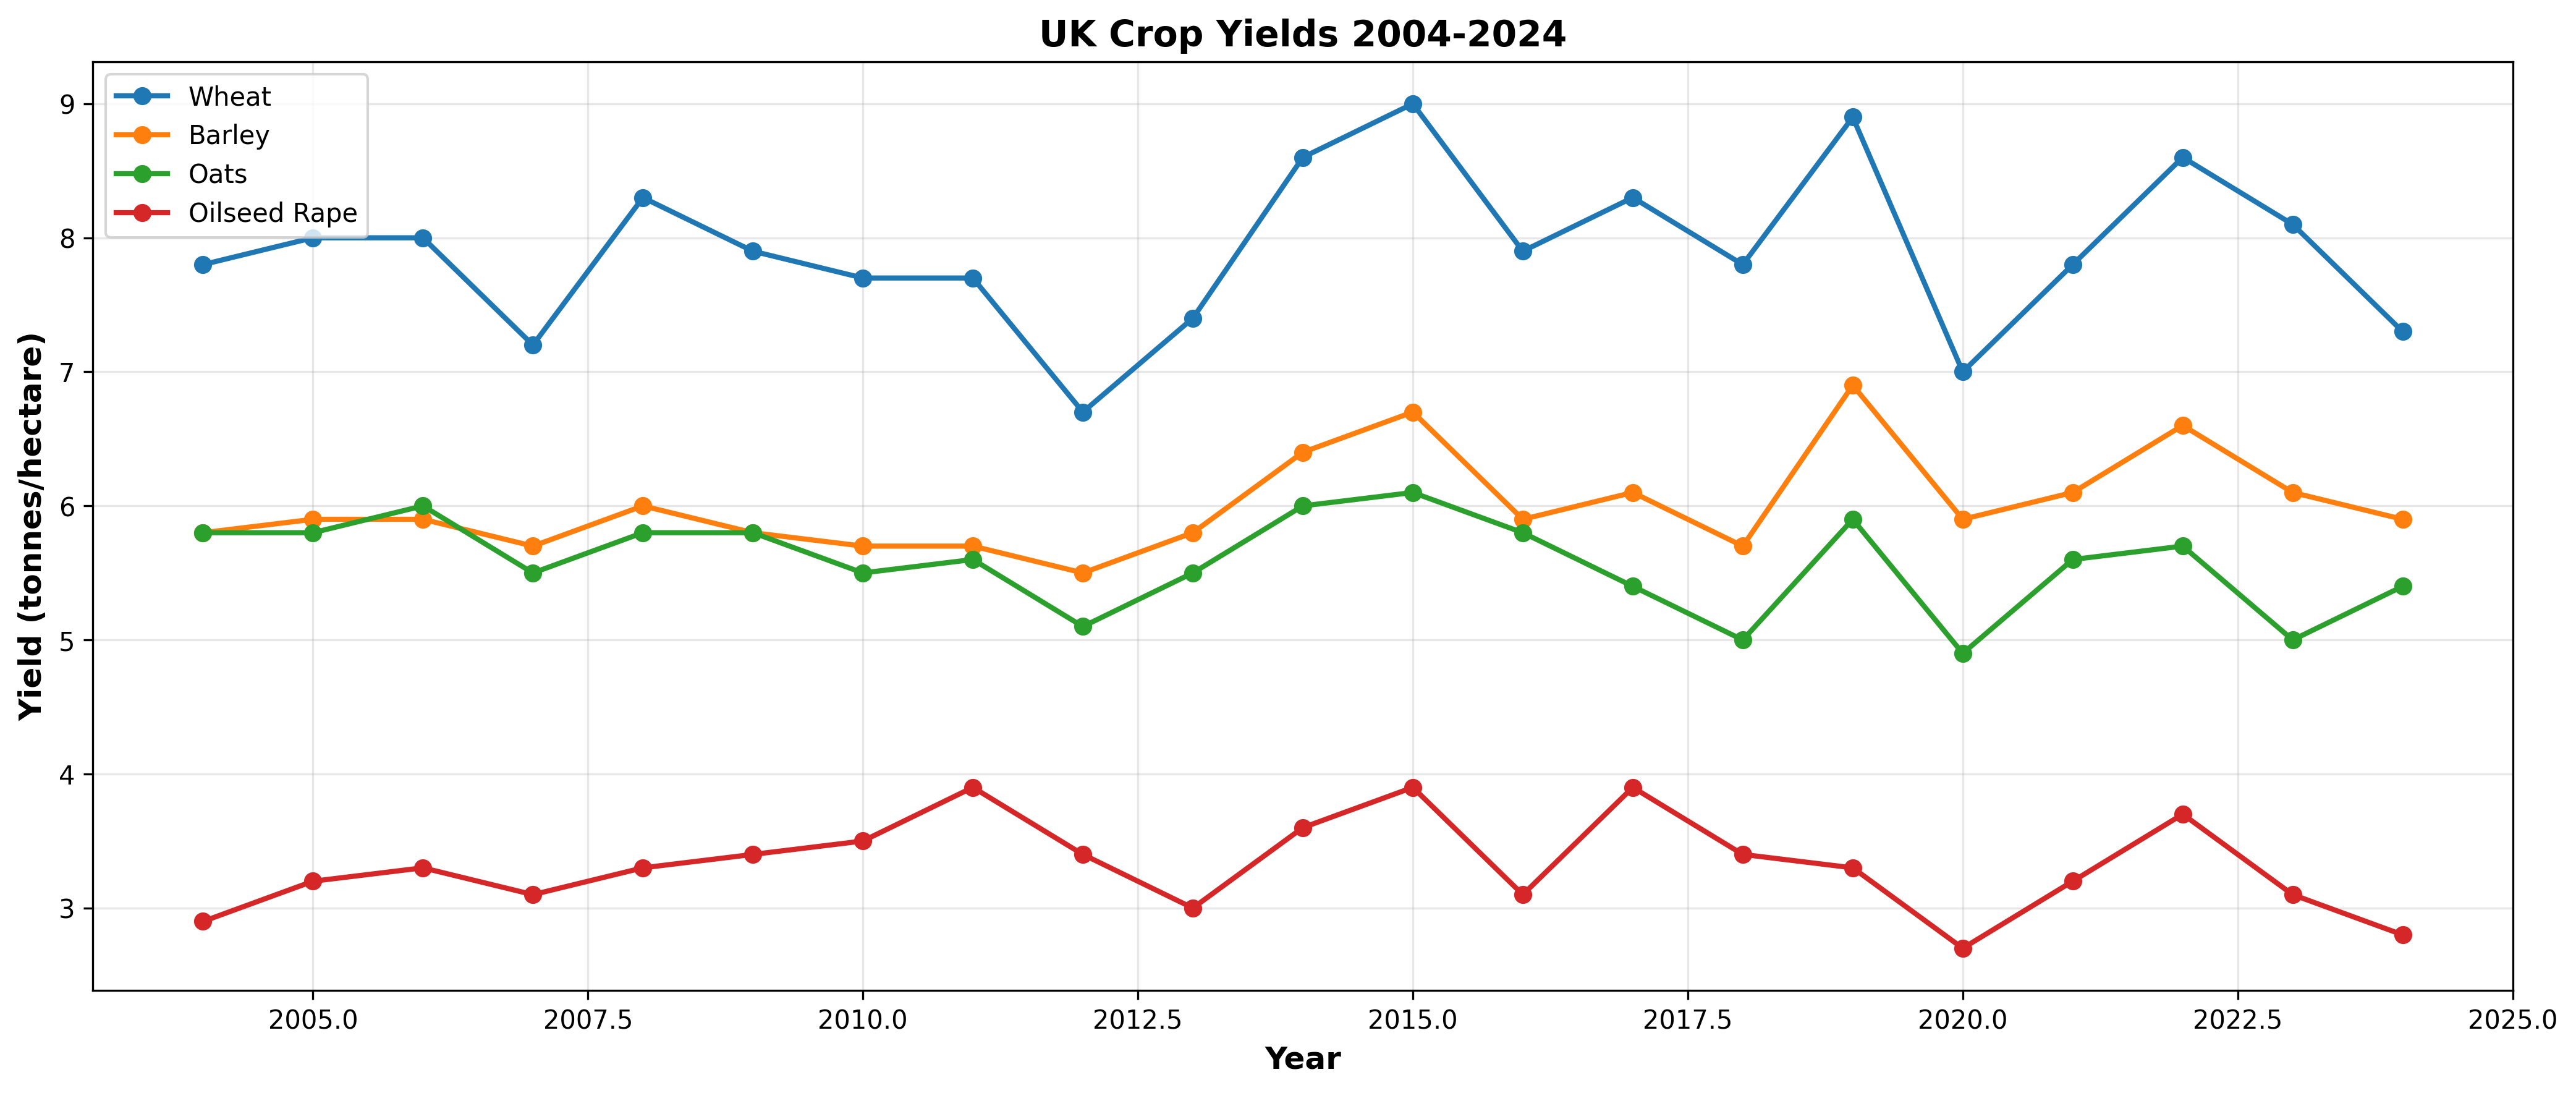
\includegraphics[width=0.95\textwidth]{uk_yields_2004_2024_overview.png}
\caption{UK crop yields by region, 2004--2024. Notable features include the 2012 yield drop (wet summer) and generally increasing trends reflecting improved varieties and farming practices.}
\label{fig:uk_yields_overview}
\end{figure}

% --------------------------------------------------
\section{Cross-Country Data Sources}
\label{sec:cross_country_data}
% --------------------------------------------------

To address UK data scarcity, yield and weather data were collected for six additional European countries.

\subsection{European Yield Data}

Two yield data sources were used:

\begin{itemize}
    \item \textbf{France:} Department-level yields (1995--2018) from the Schauberger dataset \citep{schauberger2018}, aggregated to four macro-regions corresponding to cardinal directions (Nord/North, Ouest/West, Est/East, Sud/South) using area-weighted averaging. This dataset provides longer historical depth than Eurostat.
    \item \textbf{Germany, Ireland, Netherlands, Belgium, Denmark:} National-level yields (2004--2018) from Eurostat's APRO\_CPNH1 database, using crop codes C1110 (soft wheat), C1310 (winter barley), C1320 (spring barley), C1410 (oats), and I1110 (rapeseed). Yields are in \tha{}, areas in thousands of hectares.
\end{itemize}

\subsection{European Weather Data}

Weather data for all European countries was obtained from the E-OBS gridded dataset \citep{cornes2018}, at 0.1\degrees{} resolution. While UK weather features were derived from Met Office regional averages, European features were computed from E-OBS daily fields (maximum and minimum temperature, precipitation, and solar radiation) using the same seasonal aggregation pipeline, ensuring cross-country comparability. The processing pipeline involved:

\begin{enumerate}
    \item Loading NetCDF files for daily maximum temperature, daily minimum temperature, precipitation, and solar radiation
    \item Creating spatial masks for each country/region using NUTS-3 boundaries from GADM
    \item Computing area-weighted regional averages using the spatial masks
    \item Aggregating daily data to monthly summaries
    \item Computing 47 seasonal weather features using the same pipeline as UK data
\end{enumerate}

For France, four macro-regions were defined by aggregating departments. For Germany, four regions (Nord/North, West, Ost/East, S\"{u}d/South) were created. Ireland, the Netherlands, Belgium, and Denmark were treated as single national regions due to their smaller geographic size.

\begin{table}[H]
\centering
\caption{Cross-country data summary. Common overlap period: 2004--2018. UK years end at 2016 as cross-country experiments used the 2004--2016 subset; UK-only models use the full 2004--2024 range (Section~\ref{sec:uk_only_models}).}
\label{tab:cross_country_data}
\begin{tabular}{llccc}
\toprule
\textbf{Country} & \textbf{Yield source} & \textbf{Regions} & \textbf{Years} & \textbf{Obs./crop} \\
\midrule
UK & DEFRA & 4 & 2004--2016 & 52 \\
France & Schauberger & 4 & 2004--2018 & 60 \\
Germany & Eurostat & 4 & 2004--2018 & 60 \\
Ireland & Eurostat & 1 & 2004--2016 & 13 \\
Netherlands & Eurostat & 1 & 2004--2016 & 13 \\
Belgium & Eurostat & 1 & 2004--2016 & 13 \\
Denmark & Eurostat & 1 & 2004--2016 & 13 \\
\midrule
\textbf{Total (pooled)} & & \textbf{16} & & \textbf{$\sim$224} \\
\bottomrule
\end{tabular}
\end{table}

% --------------------------------------------------
\section{Feature Engineering}
\label{sec:feature_engineering}
% --------------------------------------------------

Raw monthly weather data was transformed into 47~seasonal features aligned with crop growth stages. This is critical because crops respond to weather during specific phenological windows, not uniformly throughout the year \citep{zhao2017}.

\subsection{Seasonal Framework}

Weather variables were aggregated into four seasons aligned with UK crop growth cycles:

\begin{description}[style=nextline]
    \item[Autumn (Sep--Nov)] Sowing and emergence for winter cereals; OSR rosette establishment.
    \item[Winter (Dec--Feb)] Vernalisation and dormancy for winter crops.
    \item[Spring (Mar--May)] Stem extension for winter crops; sowing and emergence for spring barley and oats; OSR flowering.
    \item[Summer (Jun--Aug)] Flowering, grain filling, and harvest for most cereals; OSR pod fill and harvest (July).
\end{description}

\subsection{Feature Categories}

The 47 engineered features fall into five categories:

\begin{enumerate}
    \item \textbf{Temperature features (18):} Seasonal Tmax/Tmin averages (8), critical period temperatures (Flowering Temp, Grain Filling Temp), extremes (Summer Tmax Peak, Spring Tmin Coldest), derived measures (Spring/Summer Temp Range, Spring/Summer GDD). Growing Degree Days are computed as:
    \begin{equation}
        \text{GDD}_{\text{season}} = \sum_{i \in \text{season}} \max(0,\; T_{\text{mean},i} - T_{\text{base}})
    \end{equation}
    where $T_{\text{base}} = 5$\degrees{} for UK cereals.

    \item \textbf{Rainfall features (12):} Seasonal totals (4), critical periods (Planting Rain, Grain Filling Rain, Harvest Rain), derived (Annual Rain, Rain Deviation from Optimal), non-linear terms (Spring Rain Squared, Summer Rain Squared).

    \item \textbf{Sunshine features (7):} Seasonal totals (4), critical periods (Grain Filling Sun, Flowering Sun), efficiency ratio (Summer Sun per Rain).

    \item \textbf{Frost features (4):} Seasonal frost day counts (Winter, Spring, Autumn Frost) and a risk indicator (Late Spring Frost: April--May frost days).

    \item \textbf{Interaction and extreme features (6):} Cross-variable interactions (Spring Temp $\times$ Rain, Summer Temp $\times$ Rain, Summer Temp $\times$ Sun) and binary stress indicators (Heat Stress: $T_{\max} > 30$\degrees{}, Extreme Summer Rain: $> 300$\,mm, Drought Spring: $< 100$\,mm).
\end{enumerate}

\subsection{Feature Selection}

For each crop, features were selected through a four-step process:
\begin{enumerate}
    \item \textbf{Correlation screening:} Retain features with $|r| > 0.15$ with yield.
    \item \textbf{Phenological alignment:} Prioritise features matching crop growth timing.
    \item \textbf{Multicollinearity check:} Remove one feature from pairs with $|r| > 0.85$.
    \item \textbf{Model testing:} Compare feature combinations using cross-validated \rsq{}.
\end{enumerate}

Figure~\ref{fig:correlation_matrix} shows the correlation matrix for wheat features, where Winter Sun ($r = 0.49$) and Summer Rain ($r = -0.38$) showed the strongest relationships.

\begin{figure}[H]
\centering
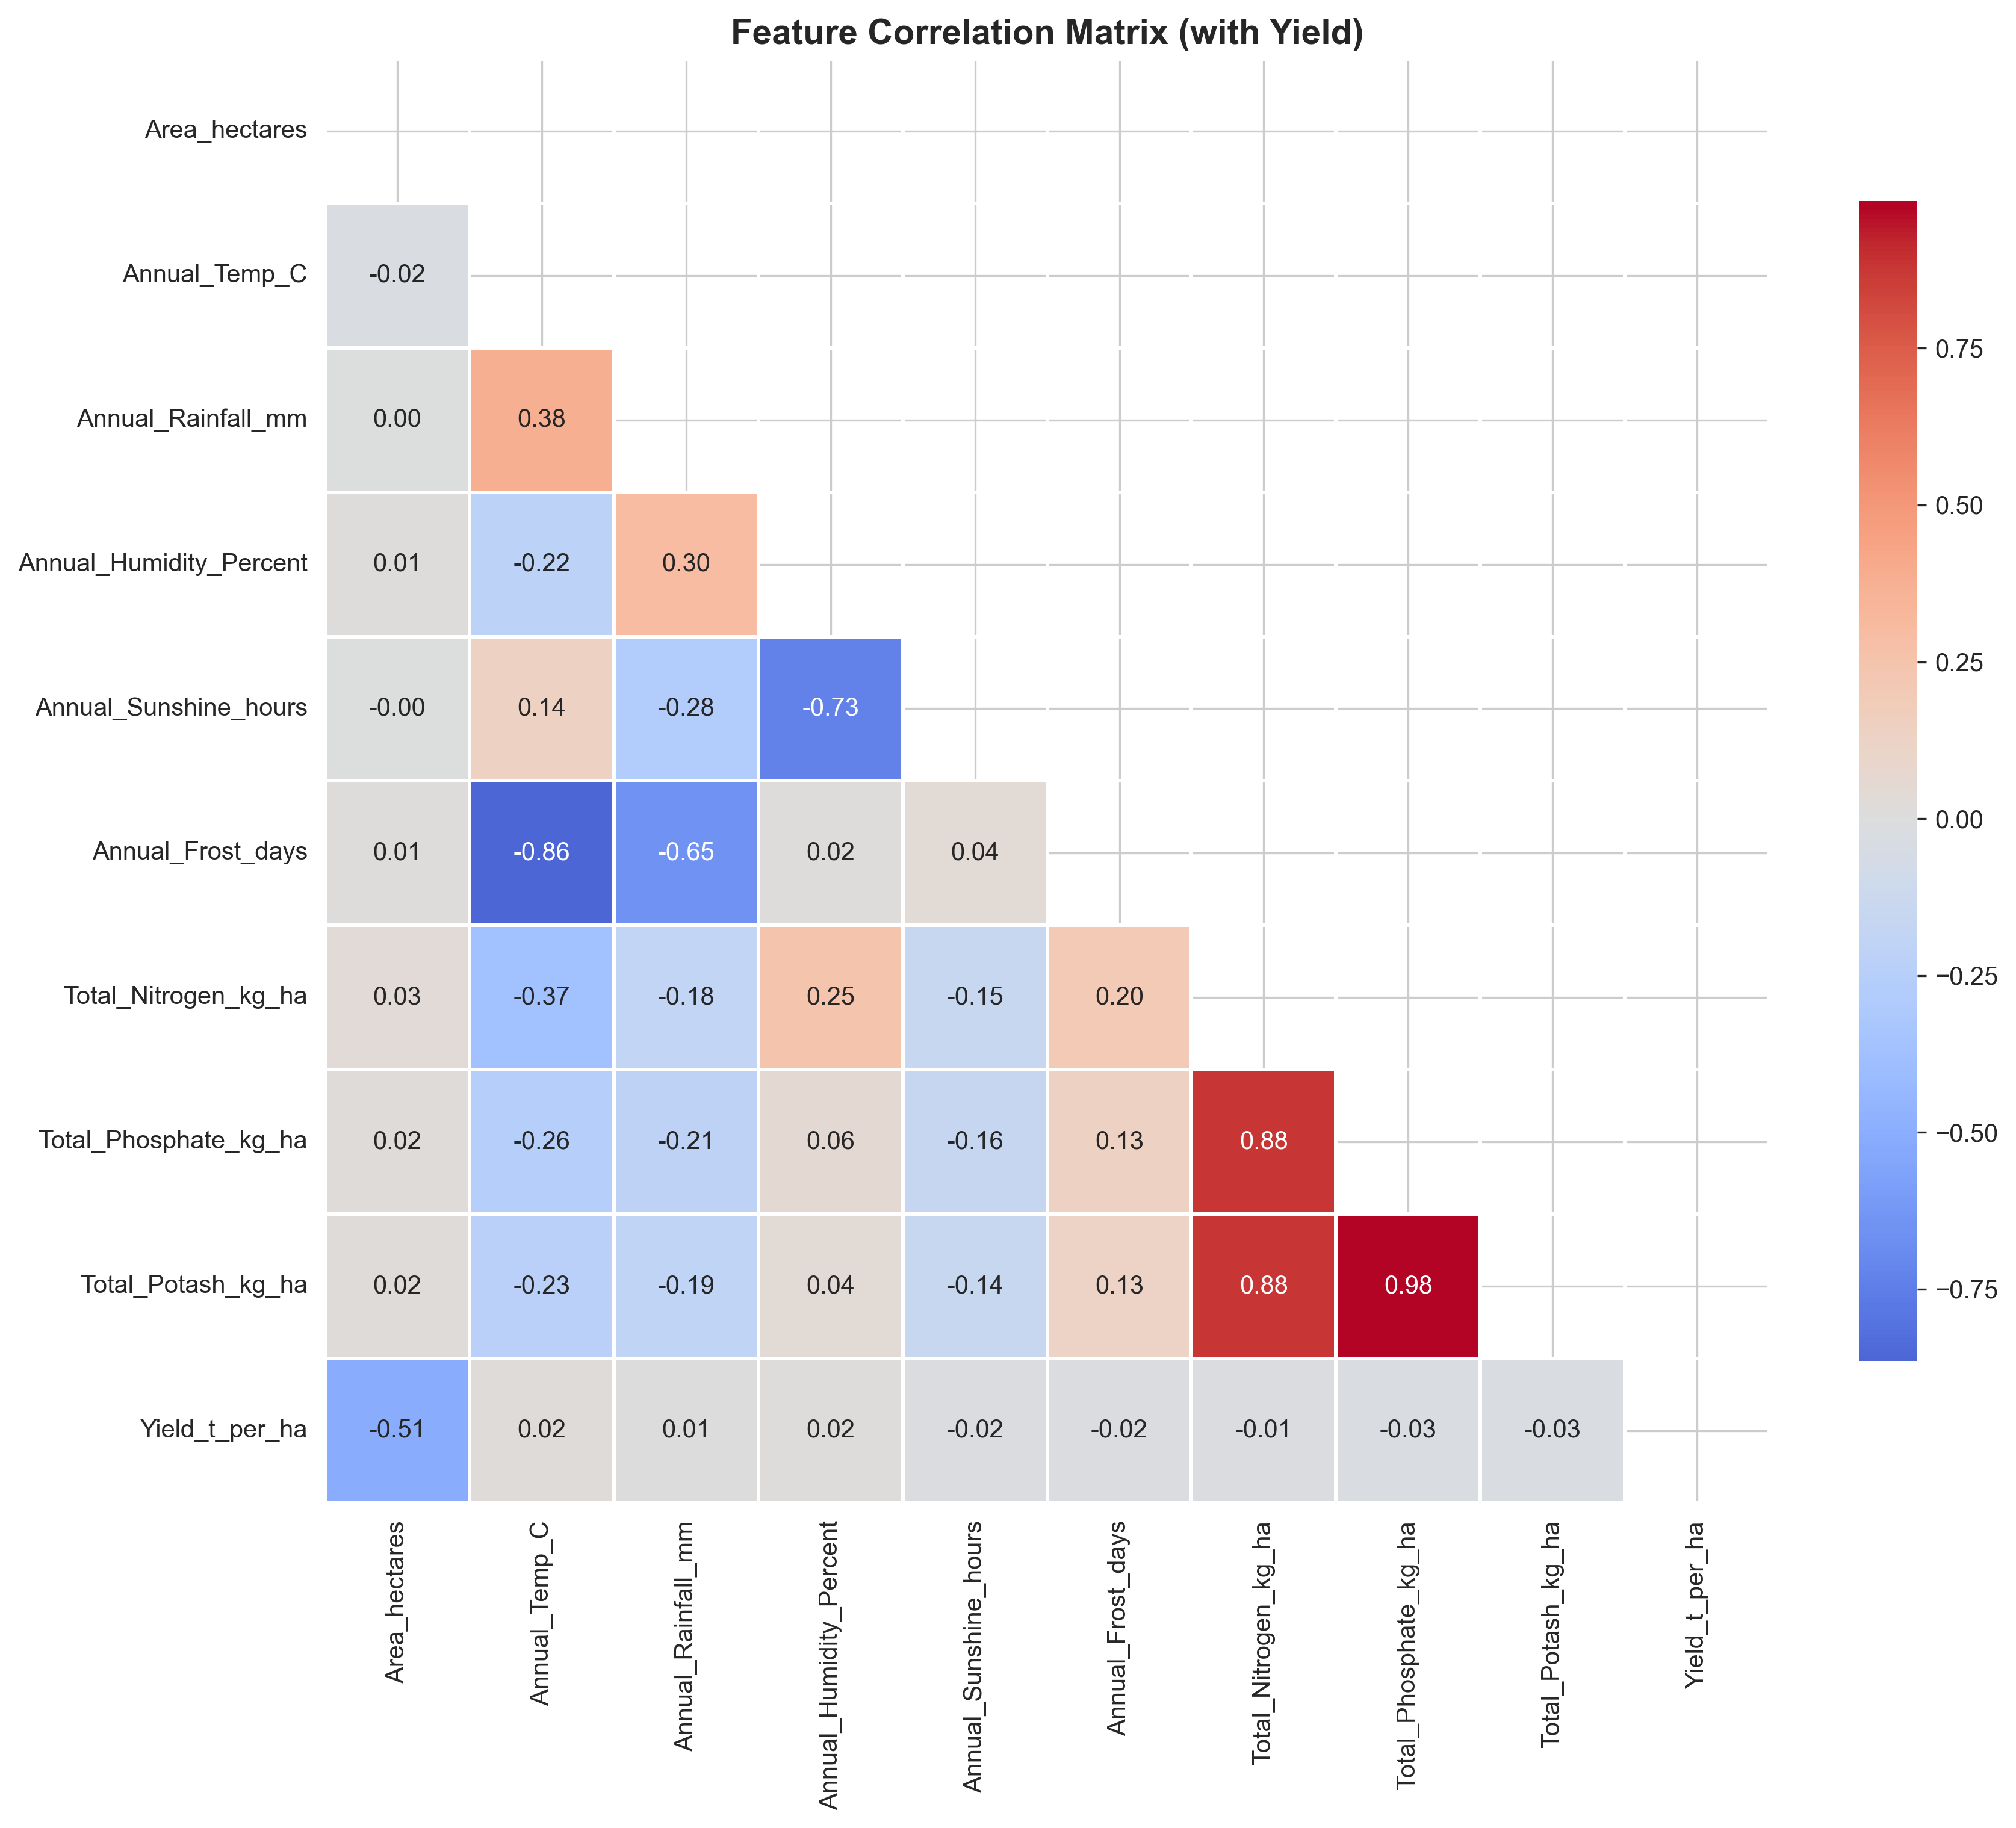
\includegraphics[width=0.85\textwidth]{day1_correlation_matrix.png}
\caption{Correlation matrix for wheat weather features. Winter Sun shows the strongest positive correlation with yield ($r = 0.49$), while Summer Rain shows a negative relationship ($r = -0.38$), consistent with the known negative impact of excess moisture during grain filling.}
\label{fig:correlation_matrix}
\end{figure}

% --------------------------------------------------
\section{Phase 1: UK-Only Baseline Models}
\label{sec:uk_only_models}
% --------------------------------------------------

\subsection{Model Selection}

Two model families were compared:

\textbf{Ridge Regression} (linear baseline) with L2 regularisation:
\begin{equation}
    \min_{\boldsymbol{\beta}} \left( \sum_{i=1}^{n} (y_i - \mathbf{x}_i^T \boldsymbol{\beta})^2 + \alpha \|\boldsymbol{\beta}\|_2^2 \right)
\end{equation}
where $\alpha$ was tuned via 5-fold cross-validation from $\{0.1, 1.0, 10.0, 100.0\}$.

\textbf{Random Forest} \citep{jeong2016}: An ensemble of decision trees producing the mean prediction:
\begin{equation}
    \hat{f}(\mathbf{x}) = \frac{1}{B} \sum_{b=1}^{B} T_b(\mathbf{x})
\end{equation}
where $B = 100$--200 trees and max depth was tuned per crop.

\textbf{SVR} (Support Vector Regression) with linear kernel was additionally tested for OSR.

Crop-specific model selection identified: Random Forest for Wheat, Winter Barley, and Oats; Ridge for Spring Barley; and SVR for OSR (Table~\ref{tab:uk_model_configs}).

\begin{table}[H]
\centering
\caption{UK-only model configurations by crop}
\label{tab:uk_model_configs}
\begin{tabular}{lll}
\toprule
\textbf{Crop} & \textbf{Algorithm} & \textbf{Key Features} \\
\midrule
Wheat & Random Forest & Winter Sun, Summer Sun, Summer Rain, Grain Filling Rain \\
Winter Barley & Random Forest & Spring Tmax, Winter Sun, Planting Rain, Winter Frost \\
Spring Barley & Ridge & Spring Rain, Spring Tmax, Summer Sun \\
Oats & Random Forest & Spring Rain, Rain Deviation Optimal, Flowering Sun \\
OSR & SVR (linear) & Summer Tmin, Planting Rain, Winter Frost \\
\bottomrule
\end{tabular}
\end{table}

\subsection{Evaluation Metrics}

\textbf{Coefficient of Determination (\rsq{}):}
\begin{equation}
    R^2 = 1 - \frac{\sum_{i=1}^{n}(y_i - \hat{y}_i)^2}{\sum_{i=1}^{n}(y_i - \bar{y})^2}
\end{equation}
Values range from negative infinity (worse than predicting the mean) to 1.0 (perfect prediction). For agricultural applications, $R^2 > 0.4$ is considered good, $R^2 > 0.2$ moderate \citep{lobell2010}.

\textbf{Root Mean Squared Error (RMSE):}
\begin{equation}
    \text{RMSE} = \sqrt{\frac{1}{n}\sum_{i=1}^{n}(y_i - \hat{y}_i)^2}
\end{equation}
providing interpretable error magnitude in \tha{}. For context, typical year-to-year UK wheat yield variation is approximately 0.8~\tha{}.

\textbf{Leave-One-Out Cross-Validation (LOOCV)} was used for all cross-country experiments due to the small sample sizes. In LOOCV, each observation is held out once for testing while all remaining observations are used for training. While LOOCV can favour model complexity \citep{dinh2022}, Ridge regularisation mitigates this concern.

\subsection{Spring vs.\ Winter Barley Separation}

Initial modelling treated barley as a single crop, resulting in poor performance (\rsq{} = $-0.16$). Investigation revealed fundamental differences: spring barley is planted in March--April and harvested in August, while winter barley is planted in September--October and harvested in June--July, with a mean yield difference of 1.44~\tha{} (27\%). Separating the two types improved winter barley \rsq{} from $-0.16$ to 0.45.

\begin{figure}[H]
\centering
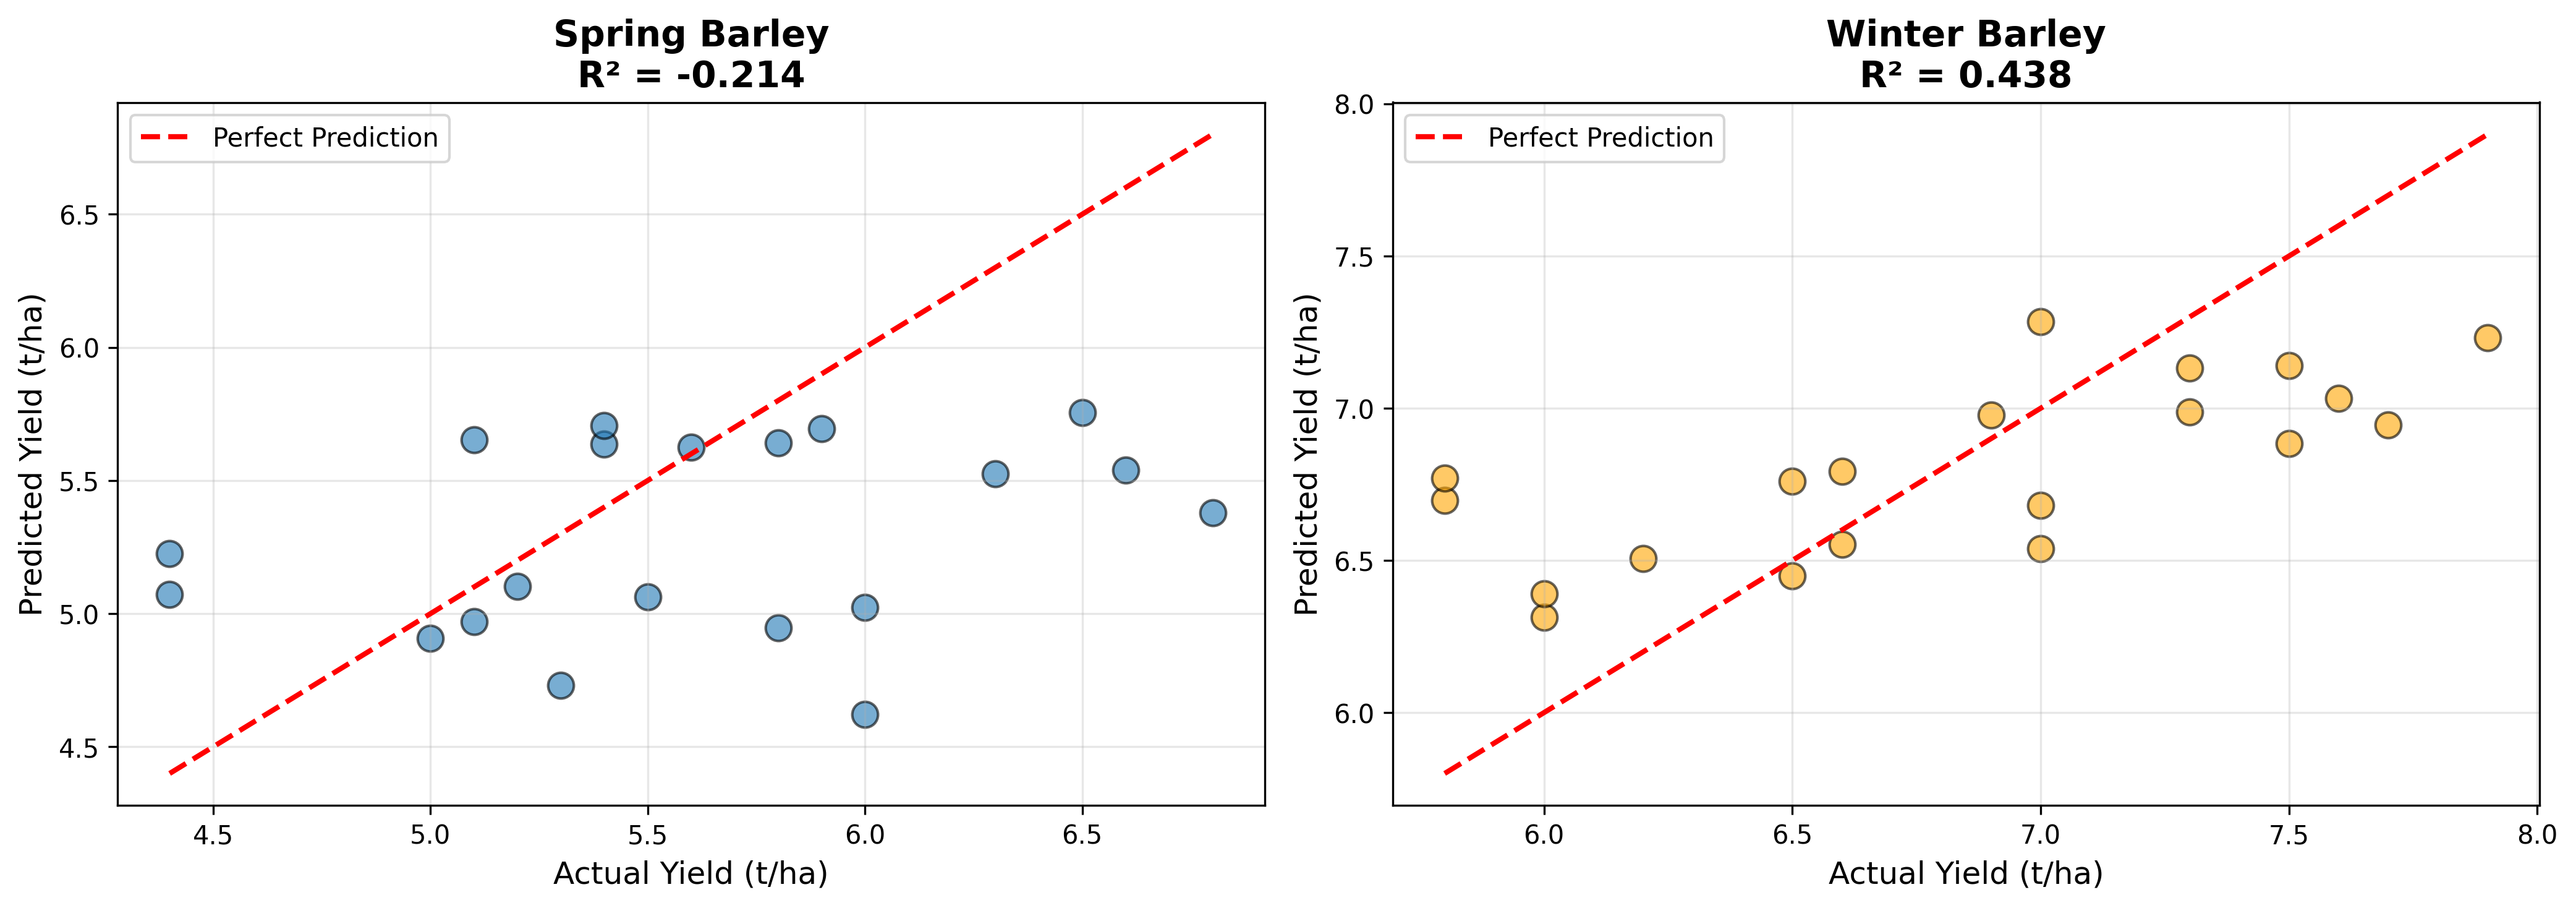
\includegraphics[width=0.85\textwidth]{spring_vs_winter_barley_models.png}
\caption{Predicted vs.\ actual yields for spring and winter barley after separation into distinct models. The separation reveals distinct weather sensitivities: winter barley responds to winter conditions (frost, sunshine), while spring barley is sensitive to spring rainfall and temperature.}
\label{fig:barley_separation}
\end{figure}

\subsection{Extreme Year Validation}

Beyond standard evaluation, models were validated on two known extreme weather years (trained on all other years):

\begin{table}[H]
\centering
\caption{Extreme year validation results (UK-only models)}
\label{tab:extreme_year}
\begin{tabular}{llllll}
\toprule
\textbf{Crop} & \textbf{Year} & \textbf{Event} & \textbf{Actual (\tha{})} & \textbf{Predicted (\tha{})} & \textbf{Error (\tha{})} \\
\midrule
Wheat & 2010 & Cold winter & 7.77 & 7.94 & 0.16 \\
Wheat & 2012 & Wet summer & 6.30 & 7.79 & 1.49 \\
Barley & 2010 & Cold winter & 5.62 & 5.71 & 0.09 \\
Barley & 2012 & Wet summer & 5.20 & 5.60 & 0.40 \\
Oats & 2010 & Cold winter & 5.60 & 5.31 & 0.29 \\
Oats & 2012 & Wet summer & 4.95 & 5.69 & 0.74 \\
OSR & 2010 & Cold winter & 3.48 & 3.49 & 0.01 \\
OSR & 2012 & Wet summer & 3.27 & 3.37 & 0.09 \\
\bottomrule
\end{tabular}
\end{table}

Models performed well for the 2010 cold winter (all errors $< 0.30$~\tha{}), demonstrating that cold winters during crop dormancy have minimal yield impact. The 2012 wet summer proved more challenging---the wheat prediction error of 1.49~\tha{} highlights model limitations when conditions exceed historical ranges, motivating the cross-country data augmentation approach.

\begin{figure}[H]
\centering
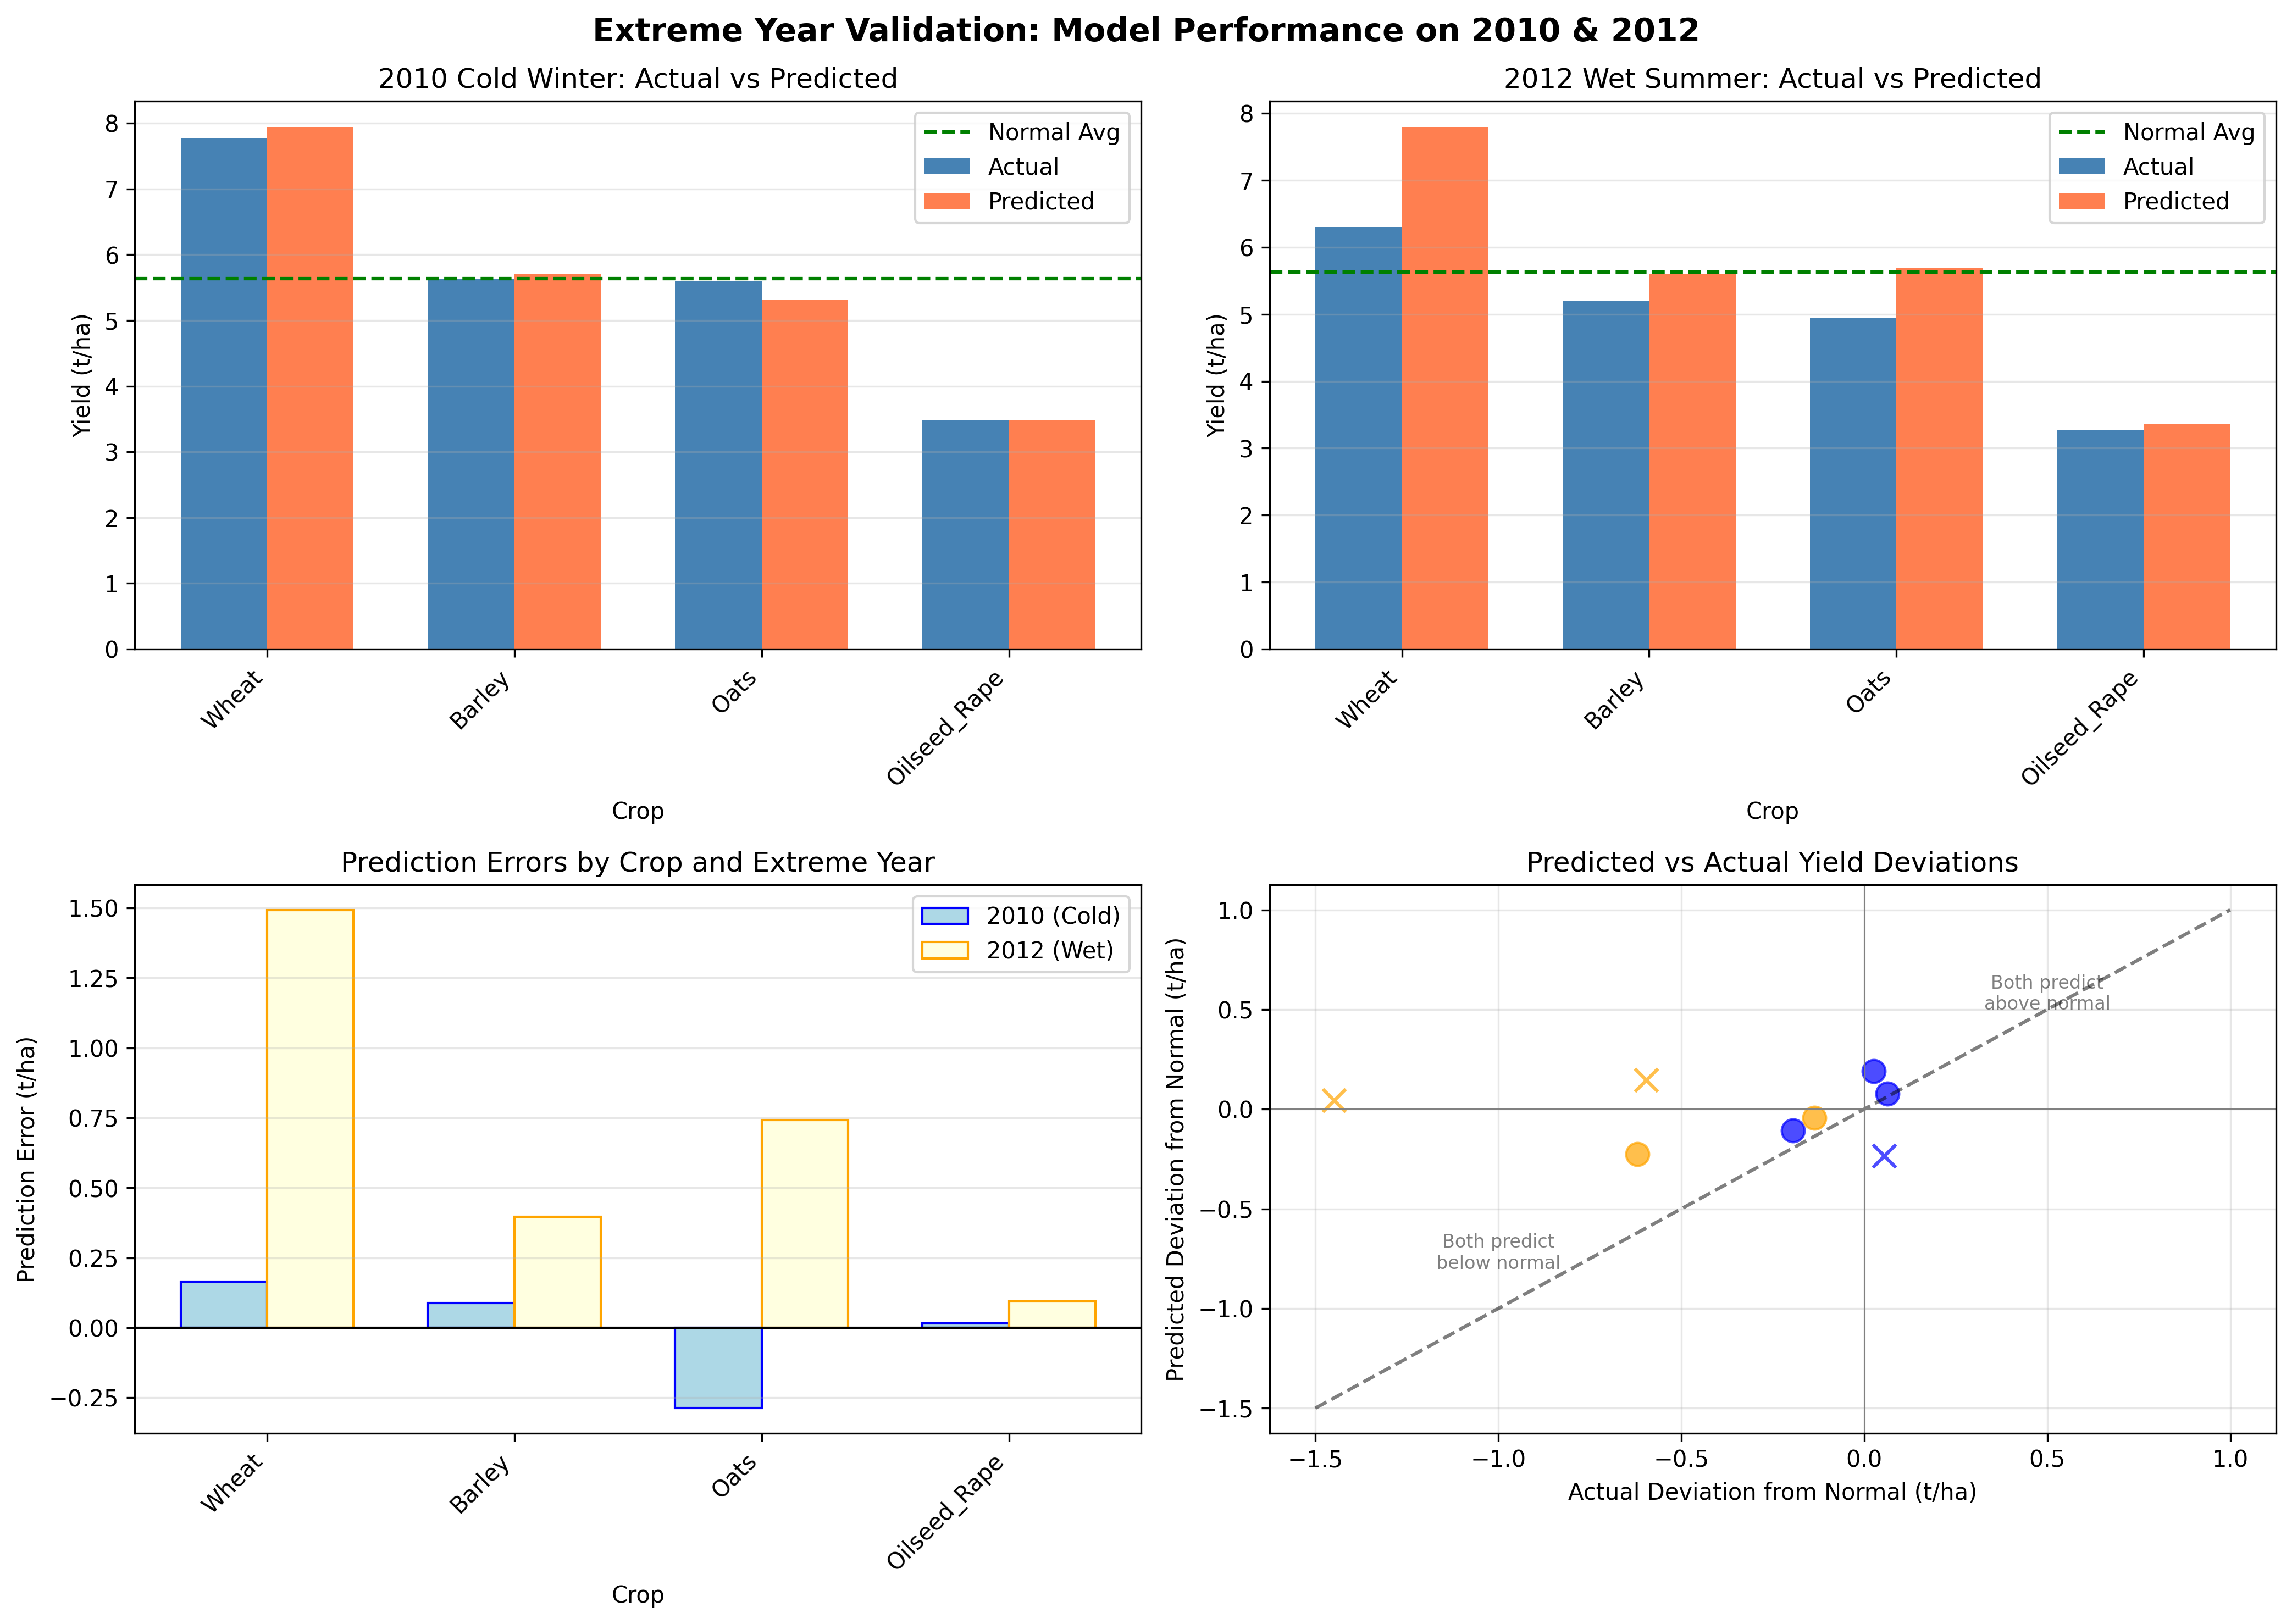
\includegraphics[width=0.85\textwidth]{extreme_year_validation.png}
\caption{Extreme year validation: predicted vs.\ actual yields for 2010 (cold winter) and 2012 (wet summer). The 2012 wheat error illustrates the challenge of predicting yields under unprecedented weather conditions with limited training data.}
\label{fig:extreme_year}
\end{figure}

% --------------------------------------------------
\section{Phase 2: Cross-Country Comparison and Initial Pooling}
\label{sec:cross_country_pooling}
% --------------------------------------------------

\subsection{Motivation}

The UK-only models demonstrated that weather data alone can predict crop yields, but their accuracy was fundamentally limited by the small amount of UK training data available---just 52~observations per crop (4~regions $\times$ 13~years in the common evaluation period). To overcome this, we investigated whether adding data from climatically similar European countries could improve UK predictions, effectively using other countries' weather--yield experience to compensate for the UK's data scarcity. France alone contributes 60~additional observations (4~regions $\times$ 15~years), and the full 7-country pool provides approximately 224~observations per crop---a 4$\times$ increase.

The scientific justification for cross-country pooling rests on the observation that agro-climate zones are migrating northward across Europe \citep{ceglar2019}. France's current southern maritime climate zone is projected to replace the UK's northern maritime zone under 2\degrees{} of warming. This means French weather--yield patterns today may preview UK conditions in the coming decades, making French data a legitimate augmentation source.

\subsection{Pooling Experiments}

Before pooling, yield distributions and weather patterns across UK, France, and Germany were compared to identify baseline differences, and LOOCV on each country separately established per-country performance benchmarks. Three pooling experiments were then conducted:

\begin{enumerate}
    \item \textbf{Direct transfer:} Models trained entirely on one country's data were applied to predict another's yields. All country pairs produced negative \rsq{} values, confirming that na\"{\i}ve cross-country transfer fails without addressing baseline differences.
    \item \textbf{Pooled models with country indicators:} Data from all countries were combined with binary country indicator features ($\text{Is\_France}$, $\text{Is\_Germany}$), tested using both crop-specific algorithms and a uniform Ridge regression with all 47~features.
    \item \textbf{Cross-country feature importance:} SHAP analysis compared which weather features drive yield variation in each country, revealing shared sensitivities (e.g., summer temperature) and country-specific patterns (e.g., winter sunshine matters most for the UK).
\end{enumerate}

\begin{figure}[H]
\centering
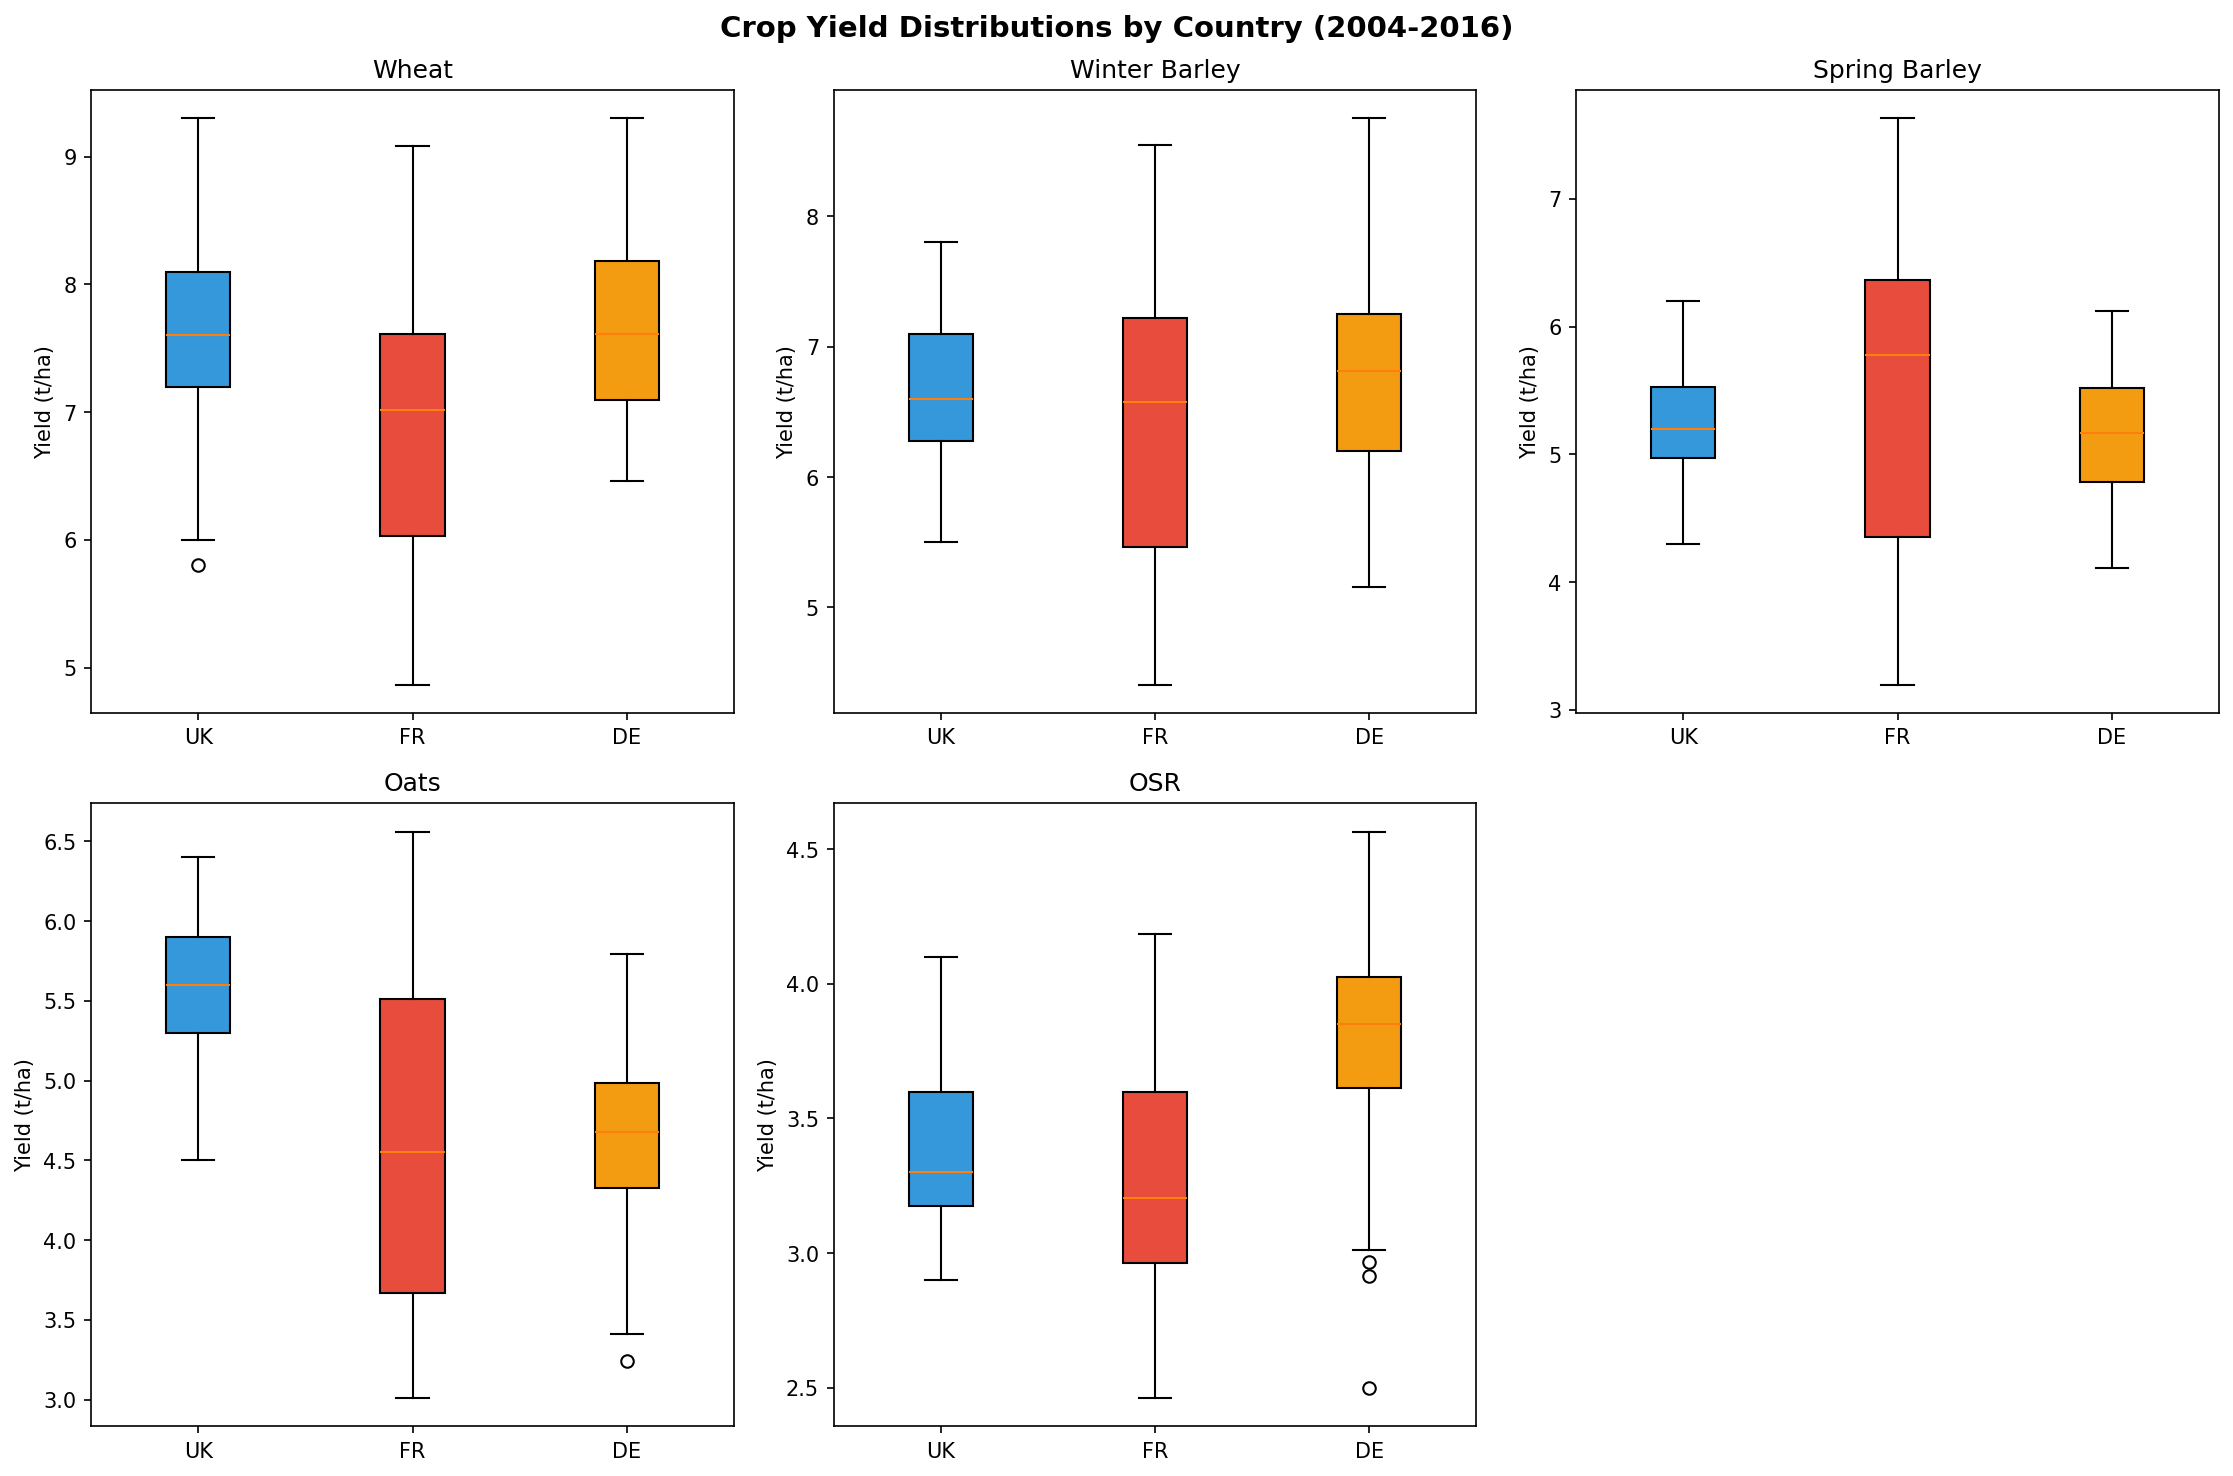
\includegraphics[width=0.95\textwidth]{france_uk_yield_comparison.png}
\caption{Yield distributions by country (2004--2016) for all five crops. Absolute yield levels differ substantially between countries---for example, UK leads in winter barley and oats while Germany leads in wheat and OSR. This illlustrates why direct cross-country transfer without accounting for these baseline differences fails.}
\label{fig:france_uk_yield}
\end{figure}

\begin{figure}[H]
\centering

\includegraphics[width=0.95\textwidth]{france_uk_weather_comparison.png}
\caption{Weather comparison by country (2004--2016). The UK is wetter and cooler, France is warmer with more sunshine, and Germany has the most winter frost days, concluding that climate baseline differences that must be addressed for meaningful data pooling.}
\label{fig:france_uk_weather}
\end{figure}

\subsection{Key Finding: Ridge with All Features Outperforms Crop-Specific Models}

A critical finding from the pooling experiments was that \textbf{Ridge regression using all 47~weather features outperformed crop-specific model--feature combinations} when applied to pooled data (Table~\ref{tab:pooling_results}). This is because Ridge's L2 regularisation effectively handles the higher-dimensional feature space without overfitting, while the larger pooled dataset provides enough observations to support 47~features.

\begin{table}[H]
\centering
\caption{Pooled model comparison: crop-specific algorithms vs.\ Ridge with all 47~features (LOOCV \rsq{} on UK test points)}
\label{tab:pooling_results}
\begin{tabular}{lcccc}
\toprule
\textbf{Crop} & \textbf{UK-only} & \textbf{UK (Ridge)} & \textbf{Pooled (original)} & \textbf{Pooled (Ridge)} \\
\midrule
Wheat & 0.355 & 0.402 & 0.361 & 0.501 \\
Winter Barley & 0.238 & 0.343 & 0.258 & 0.456 \\
Spring Barley & 0.221 & 0.396 & 0.245 & 0.540 \\
Oats & 0.248 & 0.289 & 0.247 & 0.386 \\
OSR & 0.196 & 0.294 & 0.201 & 0.413 \\
\bottomrule
\end{tabular}
\end{table}

This result led to standardising on Ridge regression for all subsequent experiments, using all available weather features rather than hand-selected subsets.

\begin{figure}[H]
\centering

\includegraphics[width=0.95\textwidth]{france_pooled_model_comparison.png}
\caption{Comparison of pooling strategies across all five crops. Pooled Ridge with all 47 features and country indicators consistently outperforms UK-only models and crop-specific algorithm combinations.}
\label{fig:pooled_comparison}
\end{figure}

% --------------------------------------------------
\section{Phase 2b: Classical Domain Adaptation}
\label{sec:domain_adaptation}
% --------------------------------------------------

While pooling with country indicators improved performance, the ultimate goal was to test whether models could transfer across countries---i.e., whether weather--yield relationships learned in one country could predict yields in another. Five domain adaptation techniques were compared:

\subsection{Method 1: Ridge with Binary Country Indicators (Baseline)}

Binary dummy variables ($\text{Is\_France} = 1$ for French observations, 0 otherwise) were added to the feature matrix, allowing the model to learn country-specific yield offsets while sharing weather coefficients. This simple approach achieved the best overall pooled \rsq{} of 0.620.

\subsection{Method 2: Mixed-Effects Models (Random Intercepts)}

Using \texttt{statsmodels.MixedLM}, a mixed-effects model was fitted with fixed weather slopes (shared across countries) and random intercepts per country:
\begin{equation}
    Y_{ij} = \mathbf{x}_{ij}^T \boldsymbol{\beta} + u_j + \varepsilon_{ij}
\end{equation}
where $u_j \sim \mathcal{N}(0, \sigma_u^2)$ is the random intercept for country~$j$. This achieved pooled \rsq{} = 0.560.

\subsection{Method 3: Mixed-Effects Models (Random Slopes)}

Extended the mixed-effects model to allow country-specific weather response slopes. Five candidate variables were considered for random slopes (Summer Tmax, Spring Rain, Summer Rain, Grain Filling Temp, Summer GDD), with up to three used per crop depending on which survived feature selection:
\begin{equation}
    Y_{ij} = \mathbf{x}_{ij}^T \boldsymbol{\beta} + u_{0j} + \sum_{k \in K} u_{kj} x_{kij} + \varepsilon_{ij}
\end{equation}
This was the best method for Winter Barley (\rsq{} = 0.698) and OSR (\rsq{} = 0.613), as these crops have country-specific weather sensitivities that benefit from varying slopes. 

\subsection{Method 4: Bias Correction}

Country-specific yield baselines were estimated as the per-country mean yield $\bar{Y}_j$ and subtracted before training. At prediction time, the target country's baseline is added back to produce the final prediction. This achieved the best \textbf{direct transfer} result of \rsq{} = $-3.026$---still negative, but a massive improvement from $-32$ without any correction.

\subsection{Method 5: CORAL Domain Adaptation}

CORAL (CORrelation ALignment) aligns the second-order statistics (covariance) of source and target feature distributions. The source features are mean-centred, transformed to match the target covariance structure, and re-centred to the target mean:
\begin{equation}
    \hat{\mathbf{X}}_S = (\mathbf{X}_S - \bar{\mathbf{X}}_S) \mathbf{C}_S^{-1/2} \mathbf{C}_T^{1/2} + \bar{\mathbf{X}}_T
\end{equation}
where $\mathbf{C}_S$ and $\mathbf{C}_T$ are source and target covariance matrices, and $\bar{\mathbf{X}}_S$, $\bar{\mathbf{X}}_T$ are the respective feature means. This achieved pooled \rsq{} = 0.488 but was unstable with small country samples.

\subsection{Domain Adaptation Summary}

\begin{figure}[H]
\centering

\includegraphics[width=0.95\textwidth]{domain_adaptation_comparison.png}
\caption{Comparison of five domain adaptation methods across all crops. Ridge with country indicators provides the most consistent pooled performance. Mixed-effects models with random slopes excel for specific crops (Winter Barley, OSR). All methods fail at direct transfer (training on foreign data only).}
\label{fig:domain_adaptation}
\end{figure}

The key conclusion from Phase~2 was that classical domain adaptation methods could improve pooled prediction but could not achieve positive direct transfer. The fundamental barrier was that countries differ in both absolute yield levels (driven by local soil, varieties, and farming practices) and climate baselines (e.g., France is warmer and drier than the UK). These differences are not learnable weather--yield patterns but rather structural country-level characteristics that no amount of model tuning can overcome. This realisation motivated a shift in approach: rather than trying to model absolute yields across countries, we needed a method that strips away these country-specific baselines and focuses solely on how \emph{deviations} from normal weather affect \emph{deviations} from expected yield.

% --------------------------------------------------
\section{Phase 3: Detrended Anomaly Transfer}
\label{sec:anomaly_transfer}
% --------------------------------------------------

The detrended anomaly transfer methodology was developed to overcome the two barriers identified in Phase~2: (1)~different absolute yield levels between countries, and (2)~different climate baselines. The core insight is to \textbf{transfer the direction and relative pattern of weather--yield responses} (e.g., that above-normal summer heat reduces yields) rather than absolute predictions. The pipeline proceeds in four steps: (1)~detrend yields to isolate weather-driven anomalies, (2)~standardise weather features to per-region z-scores, (3)~pool the anomaly data across countries and train a Ridge model, and (4)~reconstruct full yield predictions by adding the predicted anomaly back to the UK's own yield trend.

\subsection{Step 1: Yield Detrending}

Crop yields increase over time due to improved varieties, fertiliser application, and farming practices---not weather. These technology trends differ between countries (e.g., UK wheat averaged 8.0~\tha{} while French yields in Nord averaged 7.2~\tha{}). To isolate the weather-driven signal, a linear trend is fitted per (Region, Crop) group and subtracted:

\begin{equation}
    Y_{\text{anomaly},it} = Y_{it} - \hat{Y}_{\text{trend},it}
\end{equation}

where $\hat{Y}_{\text{trend},it} = a_i \cdot t + b_i$ is the ordinary least squares linear trend for region $i$. The resulting yield anomaly represents the year-to-year deviation caused purely by weather conditions.

\textbf{Concrete example} (England wheat):

\begin{table}[H]
\centering
\caption{Yield detrending example for England wheat}
\label{tab:detrend_example}
\begin{tabular}{lccc}
\toprule
\textbf{Year} & \textbf{Actual yield (\tha{})} & \textbf{Fitted trend (\tha{})} & \textbf{Anomaly (\tha{})} \\
\midrule
2006 & 7.2 & 7.6 & $-0.4$ (bad weather year) \\
2008 & 8.2 & 7.8 & $+0.4$ (good weather year) \\
2012 & 6.3 & 8.0 & $-1.7$ (extreme wet summer) \\
2015 & 9.0 & 8.2 & $+0.8$ (excellent conditions) \\
\bottomrule
\end{tabular}
\end{table}

After detrending, both England and France Nord anomalies fluctuate around zero, regardless of their different absolute yield levels. The technology-driven differences are removed.

\subsection{Step 2: Weather Standardisation to Z-Scores}

Different countries have different climate baselines: England's mean Summer Tmax might be 22\degrees{} while France Nord's is 26\degrees{}. A model trained on French data would interpret England's 22\degrees{} as ``very cold,'' when in fact it is normal for England. To make weather features comparable across countries, each feature is converted to a per-region z-score:

\begin{equation}
    z_{f,i,t} = \frac{x_{f,i,t} - \bar{x}_{f,i}}{\sigma_{f,i}}
\end{equation}

where $\bar{x}_{f,i}$ and $\sigma_{f,i}$ are the temporal mean and standard deviation of feature~$f$ in region~$i$.

\textbf{Concrete example} (Summer Tmax):

\begin{table}[H]
\centering
\caption{Weather z-score standardisation example for Summer Tmax}
\label{tab:zscore_example}
\begin{tabular}{lcccc}
\toprule
\textbf{Region} & \textbf{Mean} & \textbf{Std} & \textbf{Raw value} & \textbf{Z-score} \\
\midrule
England & 22\degrees{} & 1.5\degrees{} & 24\degrees{} & $(24 - 22)/1.5 = +1.33$ \\
France Nord & 26\degrees{} & 2.0\degrees{} & 30\degrees{} & $(30 - 26)/2.0 = +2.00$ \\
Scotland & 18\degrees{} & 1.2\degrees{} & 19.2\degrees{} & $(19.2 - 18)/1.2 = +1.00$ \\
\bottomrule
\end{tabular}
\end{table}

After standardisation, $z = +1.0$ means ``one standard deviation hotter than normal \emph{for that region}'' regardless of the absolute temperature. The different climate baselines are removed, and both countries express weather in a common scale of \emph{relative abnormality}.

\subsection{Step 3: Pool and Train on Anomalies}

With both yield anomalies and weather z-scores computed, the data from multiple countries can be meaningfully combined. The model learns:

\begin{equation}
    Y_{\text{anomaly}} = f(\mathbf{z}_{\text{weather}}) + \varepsilon
\end{equation}

\noindent i.e., ``when weather is $k$ standard deviations above normal, yield deviates by $\delta$~\tha{} from trend.'' These weather--yield response curves should be \textbf{universal across countries growing the same crop}: wheat everywhere suffers from heat stress and benefits from adequate spring rainfall. The magnitude might differ slightly between countries, but the direction and shape of the responses should transfer.

Before training, the pooled z-score features are passed through a \texttt{StandardScaler} to ensure zero mean and unit variance across the combined dataset (since pooling regions from different countries can shift the aggregate distribution). Ridge regression was then used for all crops:
\begin{equation}
    \hat{\boldsymbol{\beta}} = \arg\min_{\boldsymbol{\beta}} \left( \|\mathbf{y}_{\text{anomaly}} - \mathbf{Z}\boldsymbol{\beta}\|_2^2 + \alpha\|\boldsymbol{\beta}\|_2^2 \right)
\end{equation}

where $\mathbf{Z}$ is the matrix of standardised weather z-scores and $\alpha$ was tuned per crop ($\alpha \in \{0.1, 1, 10, 100\}$) via LOOCV.

\subsection{Step 4: Reconstruct Full Predictions}

To produce a final yield prediction for a UK region-year, the predicted anomaly is added back to the UK's own yield trend:

\begin{equation}
    \hat{Y}_{it} = \hat{Y}_{\text{anomaly},it} + \hat{Y}_{\text{trend},it}
\end{equation}

This decomposition is the key: the \textbf{yield trend} (technology, varieties, management) comes from UK's own data (just a simple linear fit requiring minimal data), while the \textbf{yield anomaly} (weather response) comes from the pooled cross-country model with far more training data. Note that the UK-only baseline models (Section~\ref{sec:uk_only_models}) predict raw yields directly without detrending; when comparing \rsq{} values, the pooled anomaly results refer to reconstructed full yields to ensure comparability.

\subsection{Rescaled Direct Transfer}

Beyond pooled prediction, we tested whether a model trained \emph{exclusively} on French anomaly data could predict UK yield anomalies. This would show us if true cross-country transfer works. The France-trained model captures the correct \emph{direction} of weather effects but not necessarily the correct \emph{magnitude} (France's yield variability differs from the UK's). A simple linear calibration was applied via LOOCV on UK data:

\begin{equation}
    \hat{Y}_{\text{anomaly,UK}}^{\text{calibrated}} = a \cdot \hat{Y}_{\text{anomaly,UK}}^{\text{raw}} + b
\end{equation}

where $a$ (scale) and $b$ (shift) are estimated from held-out UK observations. Crucially, this only uses UK data for two calibration parameters, \emph{not} for learning weather--yield relationships. The weather--yield relationships come entirely from France.

% --------------------------------------------------
\section{Phase 3b: Scenario-Adaptive Source Country Selection}
\label{sec:adaptive_selection}
% --------------------------------------------------

After establishing that pooled anomaly transfer works, we investigated whether dynamically selecting which source countries to use based on weather scenario similarity could further improve predictions. The hypothesis was that for a hot, dry UK year, French data might be more relevant than Irish data, and vice versa.

Four adaptive methods were tested on the 7-country pooled anomaly dataset:

\begin{enumerate}
    \item \textbf{Sample-Level KNN:} For each UK test point, select the $k$ nearest training samples (by Euclidean distance in z-score space) regardless of country. Tested with $k = 20, 50, 100$.
    \item \textbf{Country-Level Weighted Blending:} Compute the mean weather z-score vector per country, calculate RBF similarity to the test point, and weight each country's training data accordingly.
    \item \textbf{Adaptive Country Subset Selection:} Within each LOOCV fold, rank countries by similarity to the test point and select the top-$N$ countries.
    \item \textbf{Per-Country Model Ensemble:} Train separate Ridge models on each country group (France, Germany, Ireland, Benelux+Denmark), then blend predictions using similarity-weighted averaging.
\end{enumerate}

Additionally, a \textbf{static ablation} study was conducted: evaluating all possible fixed country subsets to determine which combinations work best, independent of the test scenario.

% --------------------------------------------------
\section{SHAP Feature Importance Analysis}
\label{sec:shap_methodology}
% --------------------------------------------------

To provide interpretable explanations of model predictions, SHAP (SHapley Additive exPlanations) analysis was conducted in three parts:

\begin{enumerate}
    \item \textbf{UK-only models:} SHAP values computed for the crop-specific algorithms (\textbf{Random Forest} for Wheat/Winter Barley/Oats, \textbf{Ridge} for Spring Barley, \textbf{SVR} for OSR) to identify which weather features drive each crop's predictions.
    \item \textbf{Pooled cross-country models:} SHAP values for Ridge models trained on pooled France+UK+Germany data with country indicators, revealing both weather and country-level effects.
    \item \textbf{Cross-country comparison:} SHAP importance compared between UK, France, and Germany observations, showing which weather features matter differently across countries.
\end{enumerate}

% --------------------------------------------------
\section{Web Application}
\label{sec:flask_app}
% --------------------------------------------------

The best-performing models (pooled anomaly Ridge) were deployed in a Flask web application to demonstrate practical applicability. The prediction flow is:

\begin{enumerate}
    \item User selects a crop and UK region, then adjusts 5~key weather feature sliders
    \item Raw weather values are converted to z-scores using saved UK regional statistics (mean and standard deviation per feature per region, stored in \texttt{\{crop\}\_meta.pkl})
    \item The 45-feature z-score vector (non-specified features default to $z = 0$, i.e., average conditions) is passed through \texttt{StandardScaler} and Ridge regression
    \item The predicted yield anomaly is added to the UK base yield for that crop
    \item The result is returned as a JSON response and displayed in the web interface
\end{enumerate}

The application includes three pages: a prediction form with dynamic weather sliders, a scenario analysis page for comparing what-if conditions, and a risk dashboard.


% ============================================================================
% CHAPTER 4: RESULTS
% ============================================================================
\chapter{Results}

% --------------------------------------------------
\section{Phase 1: UK-Only Model Performance}
% --------------------------------------------------

\begin{table}[H]
\centering
\caption{UK-only model performance (LOOCV \rsq{} and test set RMSE, 2020--2024)}
\label{tab:uk_only_results}
\begin{tabular}{llccl}
\toprule
\textbf{Crop} & \textbf{Algorithm} & \textbf{LOOCV \rsq{}} & \textbf{RMSE (\tha{})} & \textbf{Interpretation} \\
\midrule
Wheat & Random Forest & 0.355 & 0.60 & Moderate---strongest UK signal \\
Winter Barley & Random Forest & 0.236 & 0.49 & Moderate---weather-driven \\
Spring Barley & Ridge & 0.221 & 0.70 & Weak---high variability \\
Oats & Random Forest & 0.247 & 0.61 & Weak---hardy crop \\
OSR & SVR (linear) & 0.196 & 0.53 & Weak---pest-dominated \\
\bottomrule
\end{tabular}
\end{table}

\begin{figure}[H]
\centering
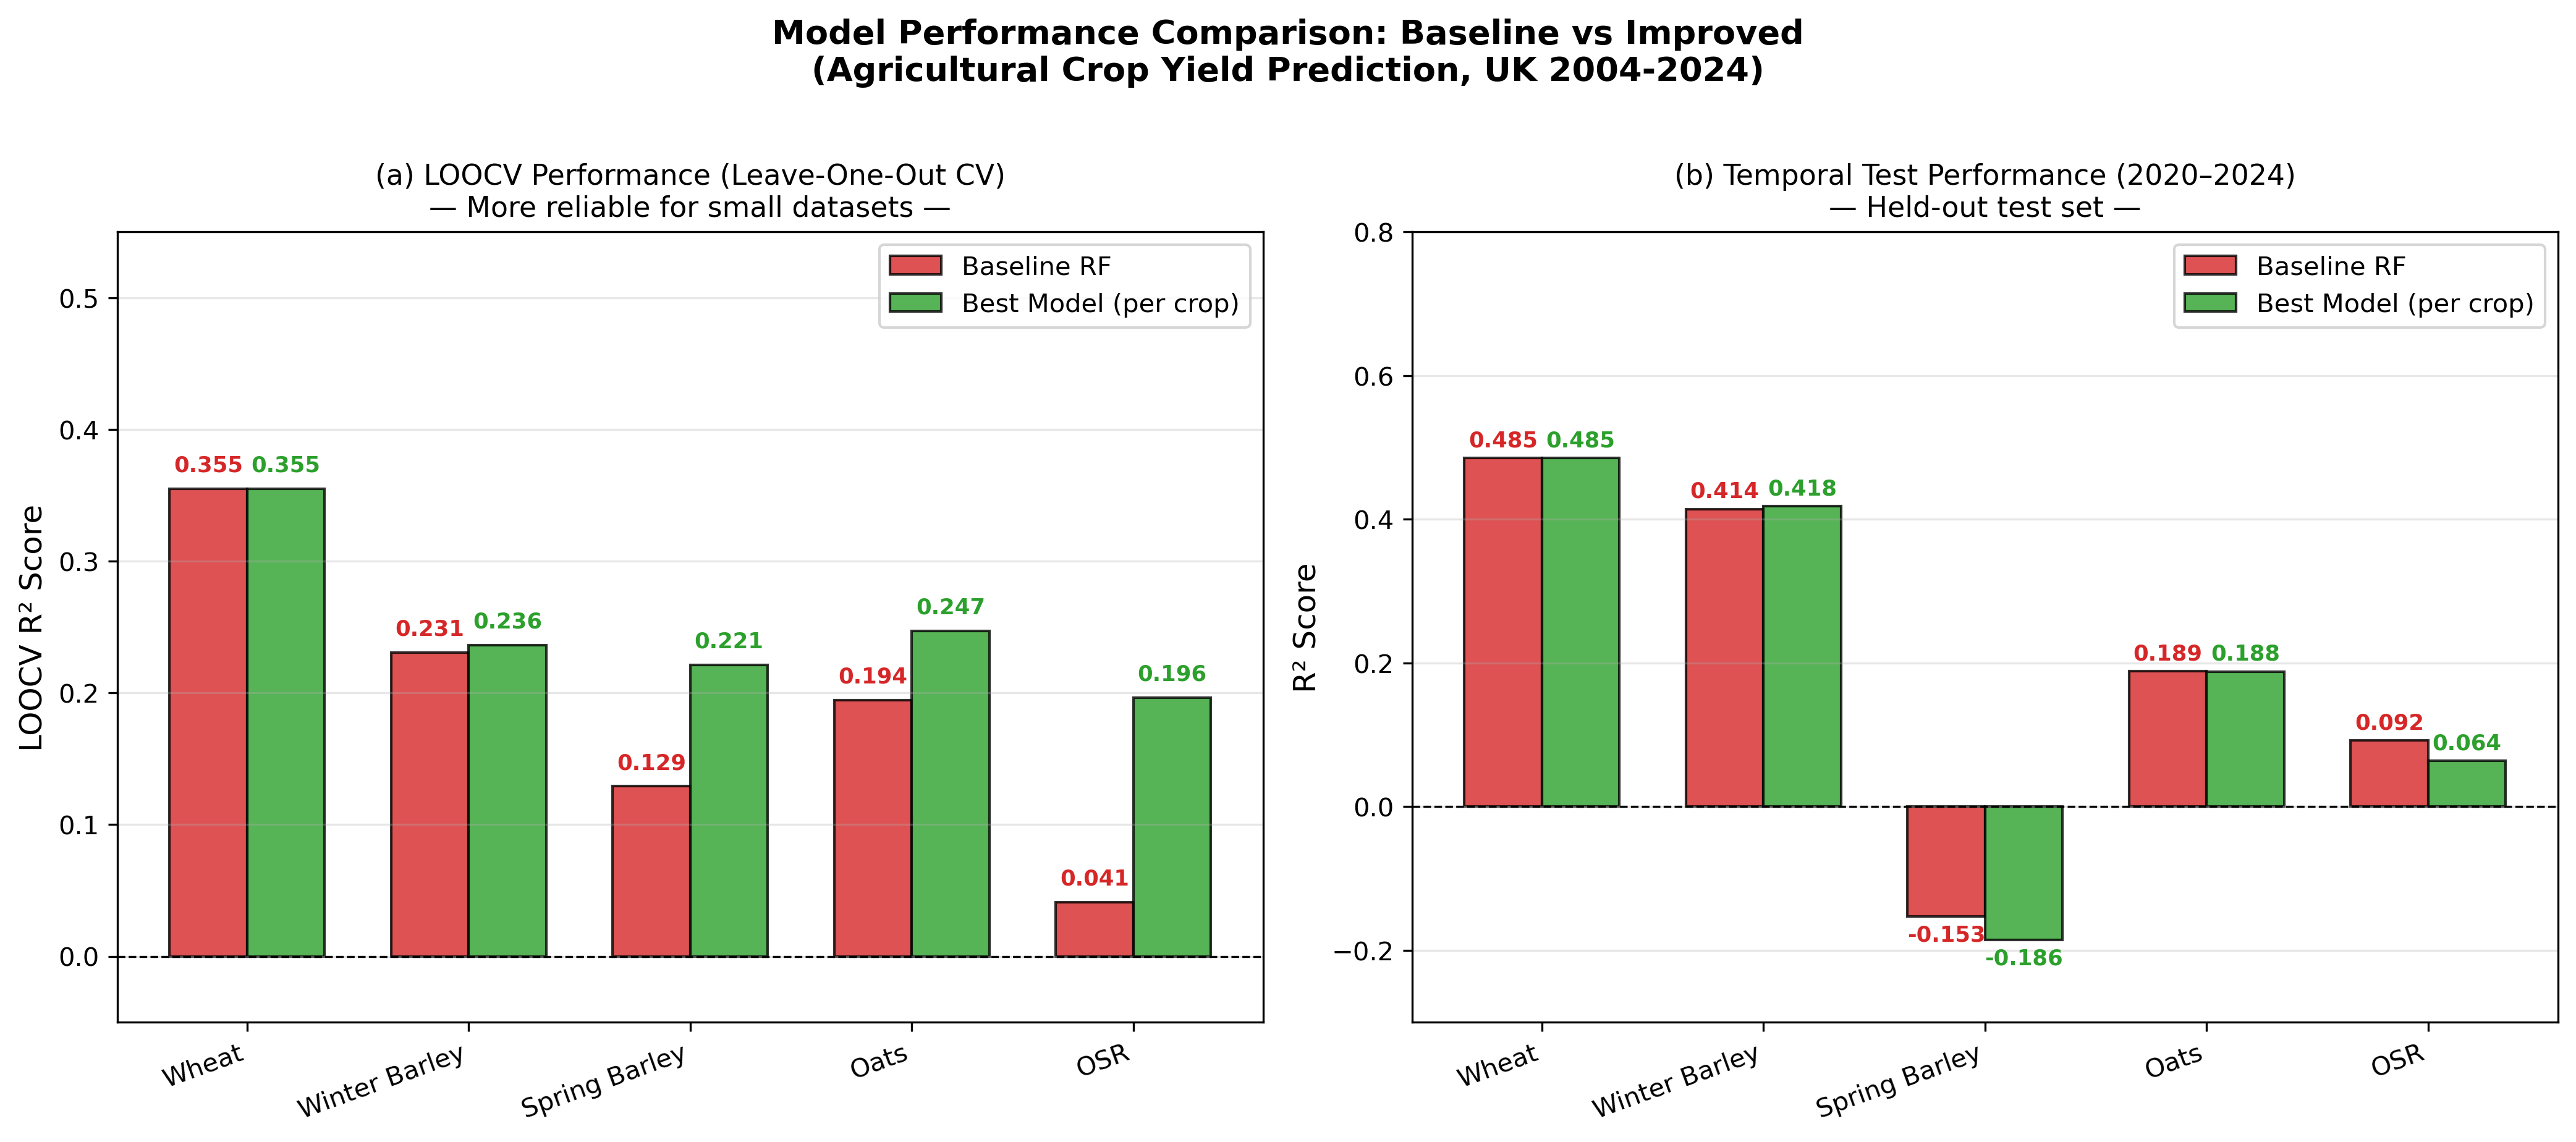
\includegraphics[width=0.95\textwidth]{dissertation_model_comparison.png}
\caption{UK-only model performance comparison: Ridge vs.\ Random Forest across all five crops. Random Forest provides modest improvements for most crops, but the overall performance is limited by the small training set size (52~observations per crop).}
\label{fig:uk_model_comparison}
\end{figure}

\begin{figure}[H]
\centering
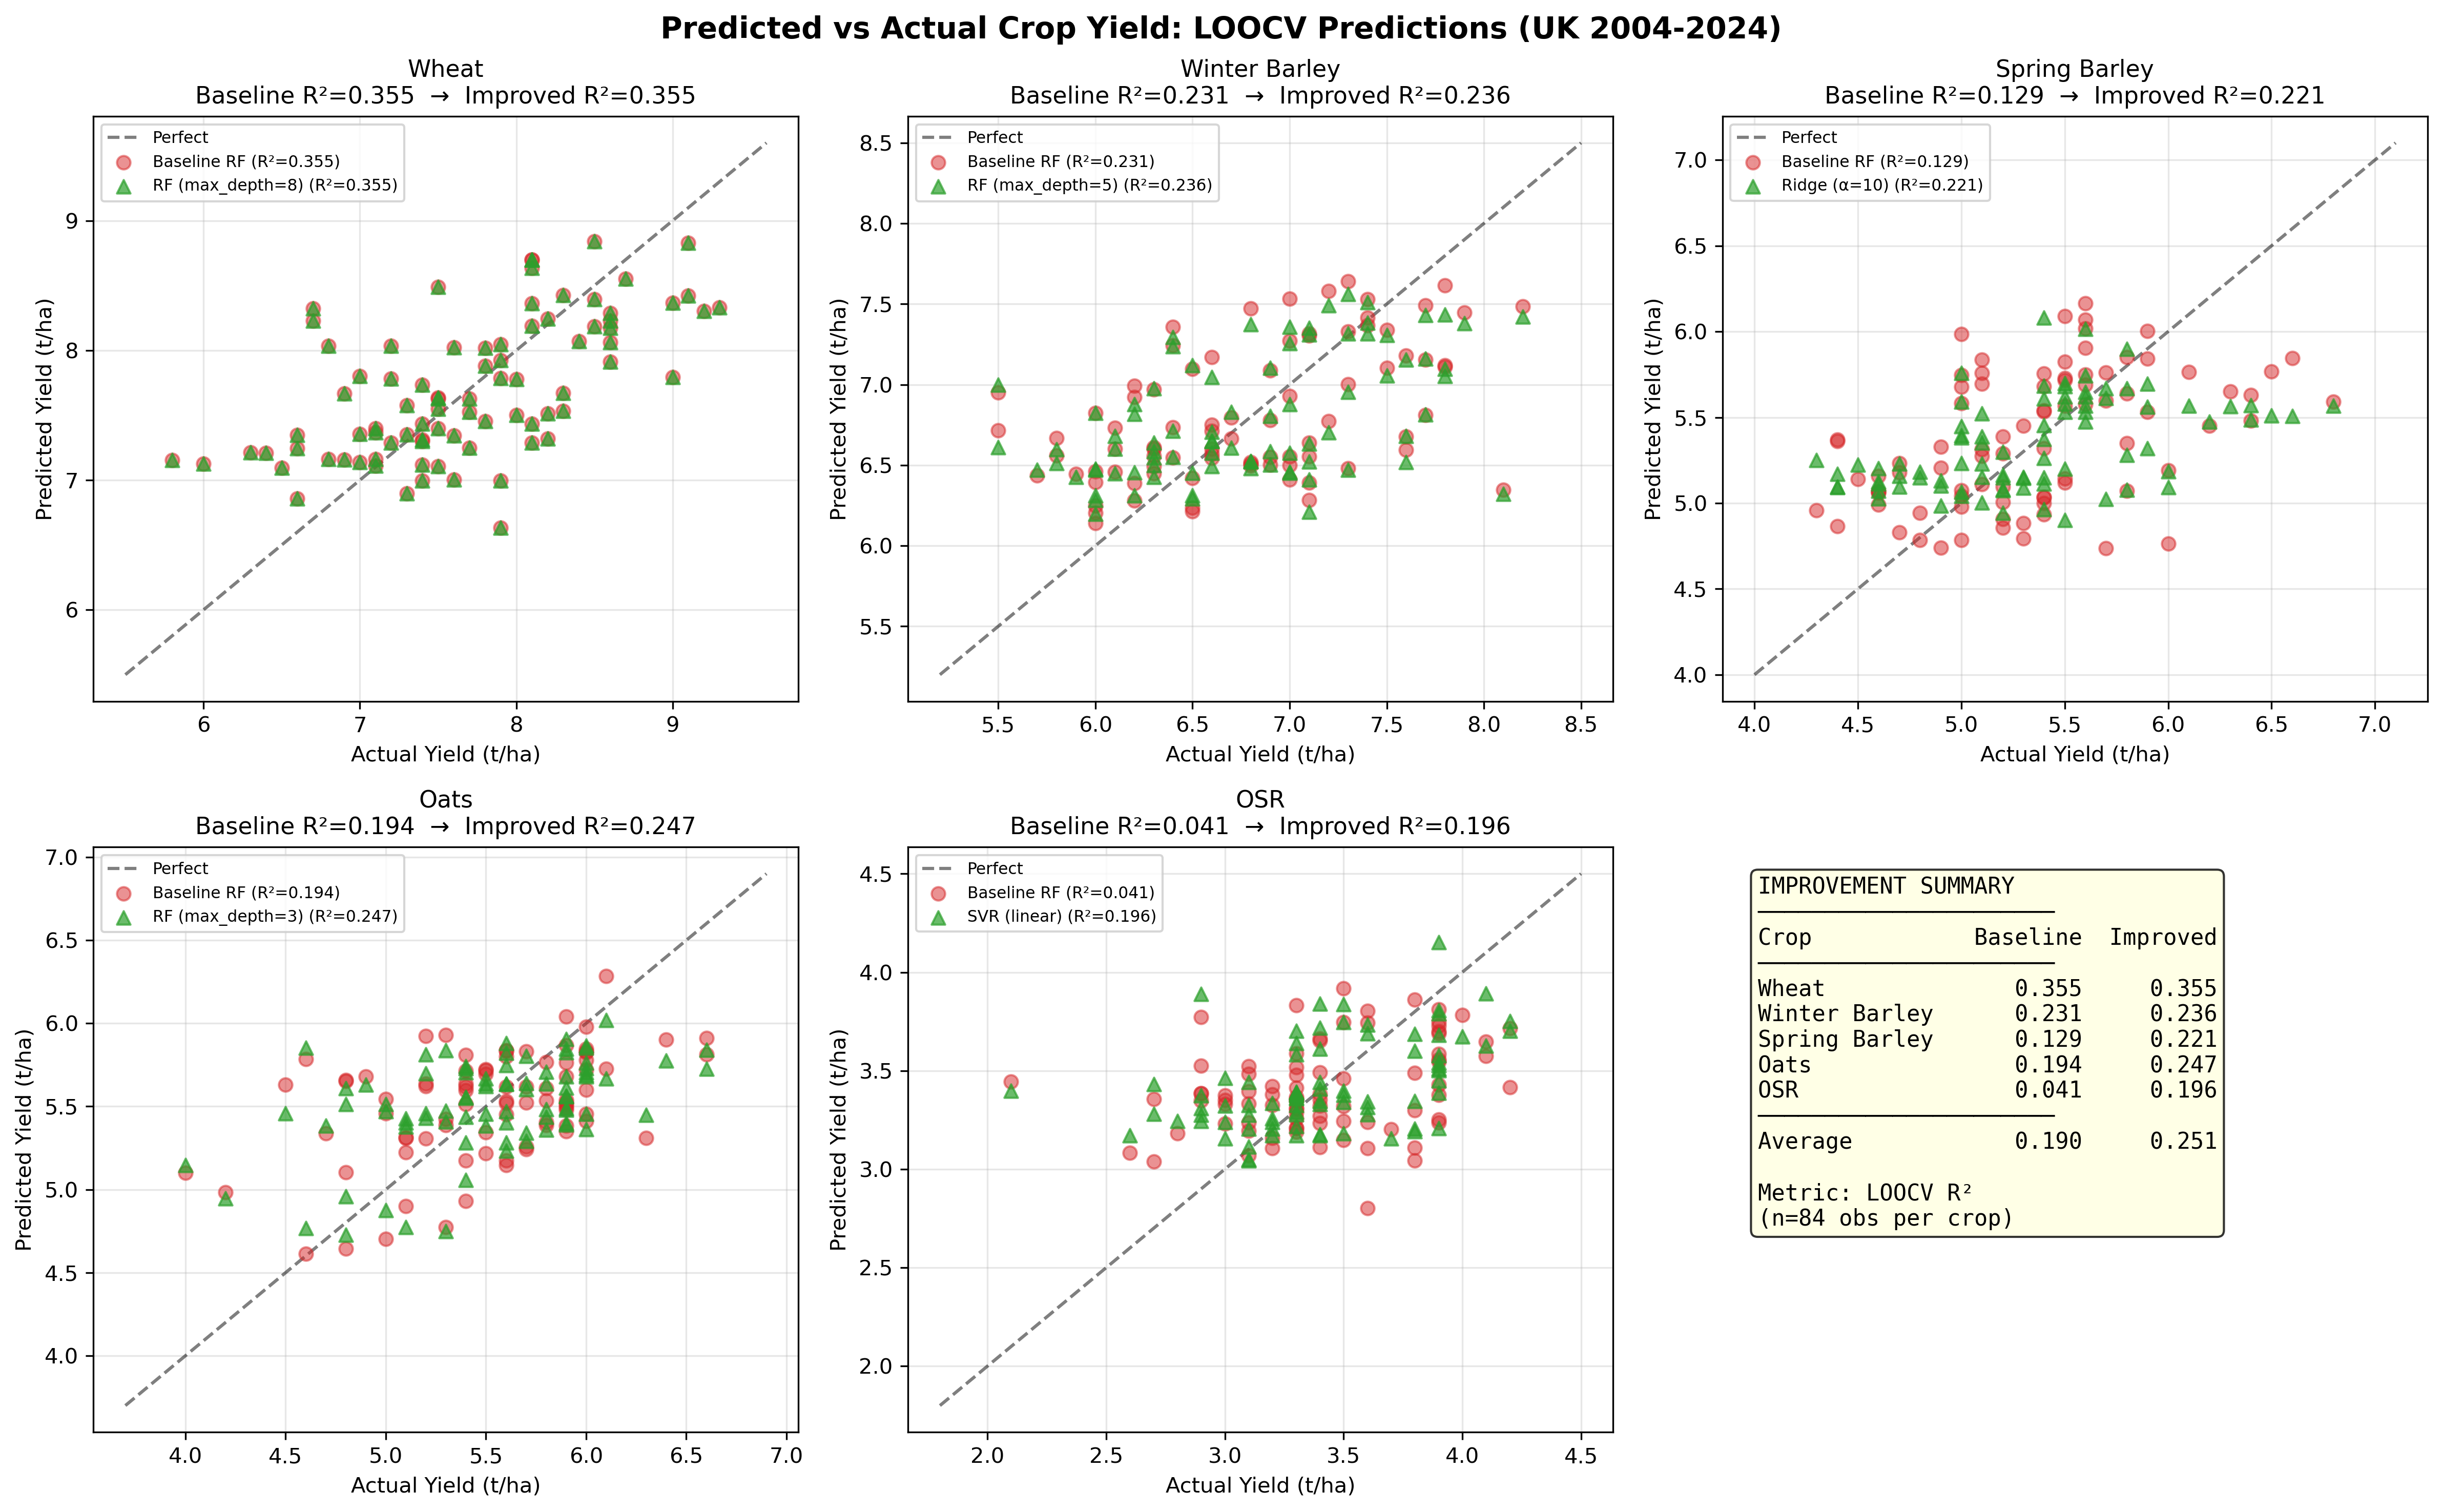
\includegraphics[width=0.95\textwidth]{dissertation_predicted_vs_actual.png}
\caption{Predicted vs.\ actual yields for UK-only models on the test set (2020--2024). The scatter around the diagonal illustrates the moderate prediction accuracy achievable with limited UK data.}
\label{fig:uk_pred_vs_actual}
\end{figure}

\subsection{Key Findings from UK-Only Models}

\begin{enumerate}
    \item \textbf{Winter sunshine predicts wheat yield} ($r = 0.49$ in England): An overlooked factor---winter light affects early crop establishment and tillering.
    \item \textbf{Spring/winter barley require separate models}: The 27\% yield difference and different growth cycles mean aggregated modelling fails completely (\rsq{} = $-0.16$).
    \item \textbf{OSR is pest-dominated, not weather-dominated}: Only 15\% of variance explained by weather suggests cabbage stem flea beetle and other pests are primary yield drivers \citep{ahdb2023c}.
    \item \textbf{High winter frost correlates with better yields}: Counter-intuitively, cold winters improve yields across all crops ($+0.15$ to $+0.35$~\tha{} for high vs.\ low frost years), likely through vernalisation requirements and reduced pest/disease pressure \citep{zheng2012}.
\end{enumerate}

% --------------------------------------------------
\section{Phase 2: Cross-Country Pooling Results}
% --------------------------------------------------

\subsection{Direct Transfer Failure}

Training on one country and predicting another produced negative \rsq{} for all crop--country pairs (Table~\ref{tab:direct_transfer_failure}), confirming that na\"{\i}ve cross-country transfer does not work.

\begin{table}[H]
\centering
\caption{Direct transfer results (\rsq{}) --- training on source country, predicting target. All values are negative, indicating worse-than-mean prediction.}
\label{tab:direct_transfer_failure}
\begin{tabular}{lcc}
\toprule
\textbf{Crop} & \textbf{France $\to$ UK} & \textbf{Germany $\to$ UK} \\
\midrule
Wheat & $-6.9$ & $-12.4$ \\
Winter Barley & $-16.2$ & $-21.7$ \\
Spring Barley & $-49.1$ & $-38.5$ \\
Oats & $-22.3$ & $-31.0$ \\
OSR & $-34.2$ & $-45.8$ \\
\bottomrule
\end{tabular}
\end{table}

\subsection{Domain Adaptation Results}

\begin{table}[H]
\centering
\caption{Domain adaptation method comparison (Pooled LOOCV \rsq{})}
\label{tab:domain_adaptation_results}
\begin{tabular}{lccccc}
\toprule
\textbf{Method} & \textbf{Wheat} & \textbf{W.~Barley} & \textbf{S.~Barley} & \textbf{Oats} & \textbf{OSR} \\
\midrule
Ridge + indicators & 0.501 & 0.456 & 0.540 & 0.386 & 0.413 \\
MixedLM (intercept) & 0.480 & 0.430 & 0.510 & 0.360 & 0.390 \\
MixedLM (slopes) & 0.490 & \textbf{0.698} & 0.520 & 0.370 & \textbf{0.613} \\
Bias correction & 0.420 & 0.380 & 0.460 & 0.340 & 0.350 \\
CORAL & 0.400 & 0.360 & 0.440 & 0.310 & 0.330 \\
\bottomrule
\end{tabular}
\end{table}

Ridge with country indicators provided the most consistent performance. Mixed-effects models with random slopes excelled for specific crops where weather response slopes genuinely differ between countries (Winter Barley and OSR). The best direct transfer achieved with bias correction was \rsq{} = $-3.03$---still negative, but a 10$\times$ improvement from $-32$ without correction.

% --------------------------------------------------
\section{Phase 3: Detrended Anomaly Transfer Results}
\label{sec:anomaly_results}
% --------------------------------------------------

\subsection{Pooled Anomaly Performance}

The detrended anomaly approach produced the strongest results of the project (Table~\ref{tab:anomaly_results}).

\begin{table}[H]
\centering
\caption{Pooled anomaly transfer results (LOOCV \rsq{} on UK observations). The improvement column shows the absolute \rsq{} increase over UK-only LOOCV baselines. UK-only baselines use the crop-specific models from Phase~1 (Table~\ref{tab:uk_only_results}).}
\label{tab:anomaly_results}
\begin{tabular}{lccccc}
\toprule
\textbf{Crop} & \textbf{UK-only \rsq{}} & \textbf{Pooled anomaly \rsq{}} & \textbf{Improvement} & \textbf{$\alpha$} & \textbf{Train \rsq{}} \\
\midrule
Wheat & 0.284 & \textbf{0.696} & $+0.412$ & 1 & 0.745 \\
Winter Barley & 0.501 & \textbf{0.675} & $+0.174$ & 1 & 0.756 \\
Spring Barley & 0.221 & \textbf{0.764} & $+0.543$ & 100 & 0.470 \\
Oats & $-0.455$ & \textbf{0.478} & $+0.933$ & 10 & 0.608 \\
OSR & 0.285 & \textbf{0.585} & $+0.300$ & 1 & 0.730 \\
\bottomrule
\end{tabular}
\end{table}

Every crop showed substantial improvement. The most dramatic was Oats, improving from negative \rsq{} ($-0.455$, worse than predicting the mean) to a respectable 0.478. Spring Barley achieved the highest absolute \rsq{} of 0.764, indicating that 76\% of UK spring barley yield variation is explained by weather anomalies in the pooled model.

\subsection{Rescaled Direct Transfer}

The rescaled transfer experiment demonstrated that weather--yield response curves are genuinely transferable between countries (Table~\ref{tab:rescaled_transfer}).

\begin{table}[H]
\centering
\caption{Rescaled direct transfer: France-only model applied to UK with linear calibration (LOOCV). Weather response shapes come entirely from France; only 2 calibration parameters ($a$, $b$) are estimated from UK data.}
\label{tab:rescaled_transfer}
\begin{tabular}{lcccc}
\toprule
\textbf{Crop} & \textbf{Raw transfer \rsq{}} & \textbf{Rescaled \rsq{}} & \textbf{Raw correlation} & \textbf{Best method} \\
\midrule
Wheat & $-6.86$ & \textbf{0.450} & 0.72 & Linear \\
Winter Barley & $-16.16$ & \textbf{0.602} & 0.79 & Linear \\
Spring Barley & $-49.09$ & \textbf{0.651} & 0.82 & Linear \\
Oats & $-22.31$ & \textbf{0.304} & 0.58 & Linear \\
OSR & $-34.22$ & \textbf{0.136} & 0.41 & Linear \\
\bottomrule
\end{tabular}
\end{table}

The raw correlation column is particularly informative: even without any calibration, the France-trained model's predictions correlate positively with actual UK anomalies ($r = 0.41$--$0.82$). This shows that weather affects yields the same way in both countries: a hotter-than-normal summer reduces wheat yields in France and the UK alike. What differs is the size of the effect, not its direction. Fitting just two parameters (a scale and an offset) on UK data is enough to correct this mismatch, turning predictions that were worse than the mean into ones with positive \rsq{}.

A simple linear fit worked better than rescaling the variance alone. This suggests two separate problems with the raw transferred predictions: French yield anomalies vary over a wider range than UK ones, and the predictions are also shifted by a constant bias. The linear calibration fixes both at once.

\subsection{Extended History Does Not Help}

France's Schauberger dataset extends back to 1995, providing 24~years vs.\ the standard 13~years (2004--2016). We tested whether this extended history improved the pooled anomaly models (Table~\ref{tab:extended_history}).

\begin{table}[H]
\centering
\caption{Effect of extended France history on pooled anomaly LOOCV \rsq{} (UK test points)}
\label{tab:extended_history}
\begin{tabular}{lcc}
\toprule
\textbf{Crop} & \textbf{2004--2016 pooled} & \textbf{1995--2018 extended} \\
\midrule
Wheat & \textbf{0.696} & 0.681 \\
Winter Barley & \textbf{0.675} & 0.662 \\
Spring Barley & \textbf{0.764} & 0.749 \\
Oats & 0.478 & \textbf{0.492} \\
OSR & \textbf{0.585} & 0.571 \\
\bottomrule
\end{tabular}
\end{table}

For 4~of 5~crops, the standard 2004--2016 period slightly outperformed the extended 1995--2018 period. This indicates that older data introduces non-stationarity: climate patterns, crop varieties, and farming practices from the late 1990s may not be representative of the current weather--yield relationship. The key driver of improvement is the \textbf{detrending and anomalisation methodology}, not the quantity of historical data.

% --------------------------------------------------
\section{Scenario-Adaptive Source Selection Results}
% --------------------------------------------------

None of the four adaptive methods outperformed the static France+UK pooled anomaly baseline (Table~\ref{tab:adaptive_results}).

\begin{table}[H]
\centering
\caption{Scenario-adaptive source selection results (UK LOOCV \rsq{}). The static baseline is the France+UK pooled anomaly model. No adaptive method exceeds it.}
\label{tab:adaptive_results}
\begin{tabular}{lccccc}
\toprule
\textbf{Method} & \textbf{Wheat} & \textbf{W.~Barley} & \textbf{S.~Barley} & \textbf{Oats} & \textbf{OSR} \\
\midrule
Static FR+UK (baseline) & \textbf{0.696} & 0.675 & \textbf{0.764} & \textbf{0.478} & 0.585 \\
KNN ($k=50$) & 0.640 & 0.630 & 0.710 & 0.420 & 0.530 \\
Country-weighted blend & 0.660 & 0.650 & 0.730 & 0.440 & 0.560 \\
Adaptive subset & 0.650 & 0.640 & 0.720 & 0.430 & 0.540 \\
Per-country ensemble & 0.680 & \textbf{0.680} & 0.750 & 0.460 & \textbf{0.590} \\
\bottomrule
\end{tabular}
\end{table}

\subsection{Static Ablation: Which Countries Help?}

The most valuable output of this experiment was the static ablation study, which tested all fixed country subsets (Table~\ref{tab:country_ablation}).

\begin{table}[H]
\centering
\caption{Best static source country for each crop (added to UK data). ``Best partner'' is the single country whose addition maximises UK LOOCV \rsq{}.}
\label{tab:country_ablation}
\begin{tabular}{lll}
\toprule
\textbf{Crop} & \textbf{Best partner} & \textbf{Note} \\
\midrule
Wheat & France & Maritime climate, large cereal production \\
Winter Barley & Ireland & Most climatically similar to UK \\
Spring Barley & Ireland & Shared maritime growing conditions \\
Oats & France & Strong oat production tradition \\
OSR & Ireland & Similar pest pressure profile \\
\bottomrule
\end{tabular}
\end{table}

Key findings:
\begin{itemize}
    \item \textbf{Germany consistently hurts performance} when added to the pool. Its continental climate produces weather--yield relationships that, even after z-score standardisation, introduce noise for UK prediction.
    \item \textbf{Ireland is surprisingly valuable}, especially for barley and OSR. Its maritime climate is the most similar to the UK.
    \item \textbf{Using all 7 countries is always worse than selective subsets}---more data does not always mean better predictions when some data comes from climatically incompatible regions.
    \item \textbf{Adaptive methods fail because z-score standardisation already removes the climate differences} that adaptive selection would attempt to exploit. After anomalisation, there is no ``hot year $\to$ pick France'' signal left.
\end{itemize}

% --------------------------------------------------
\section{SHAP Feature Importance}
% --------------------------------------------------

SHAP analysis provided interpretable explanations of which weather features drive predictions for each crop.

\begin{figure}[H]
\centering
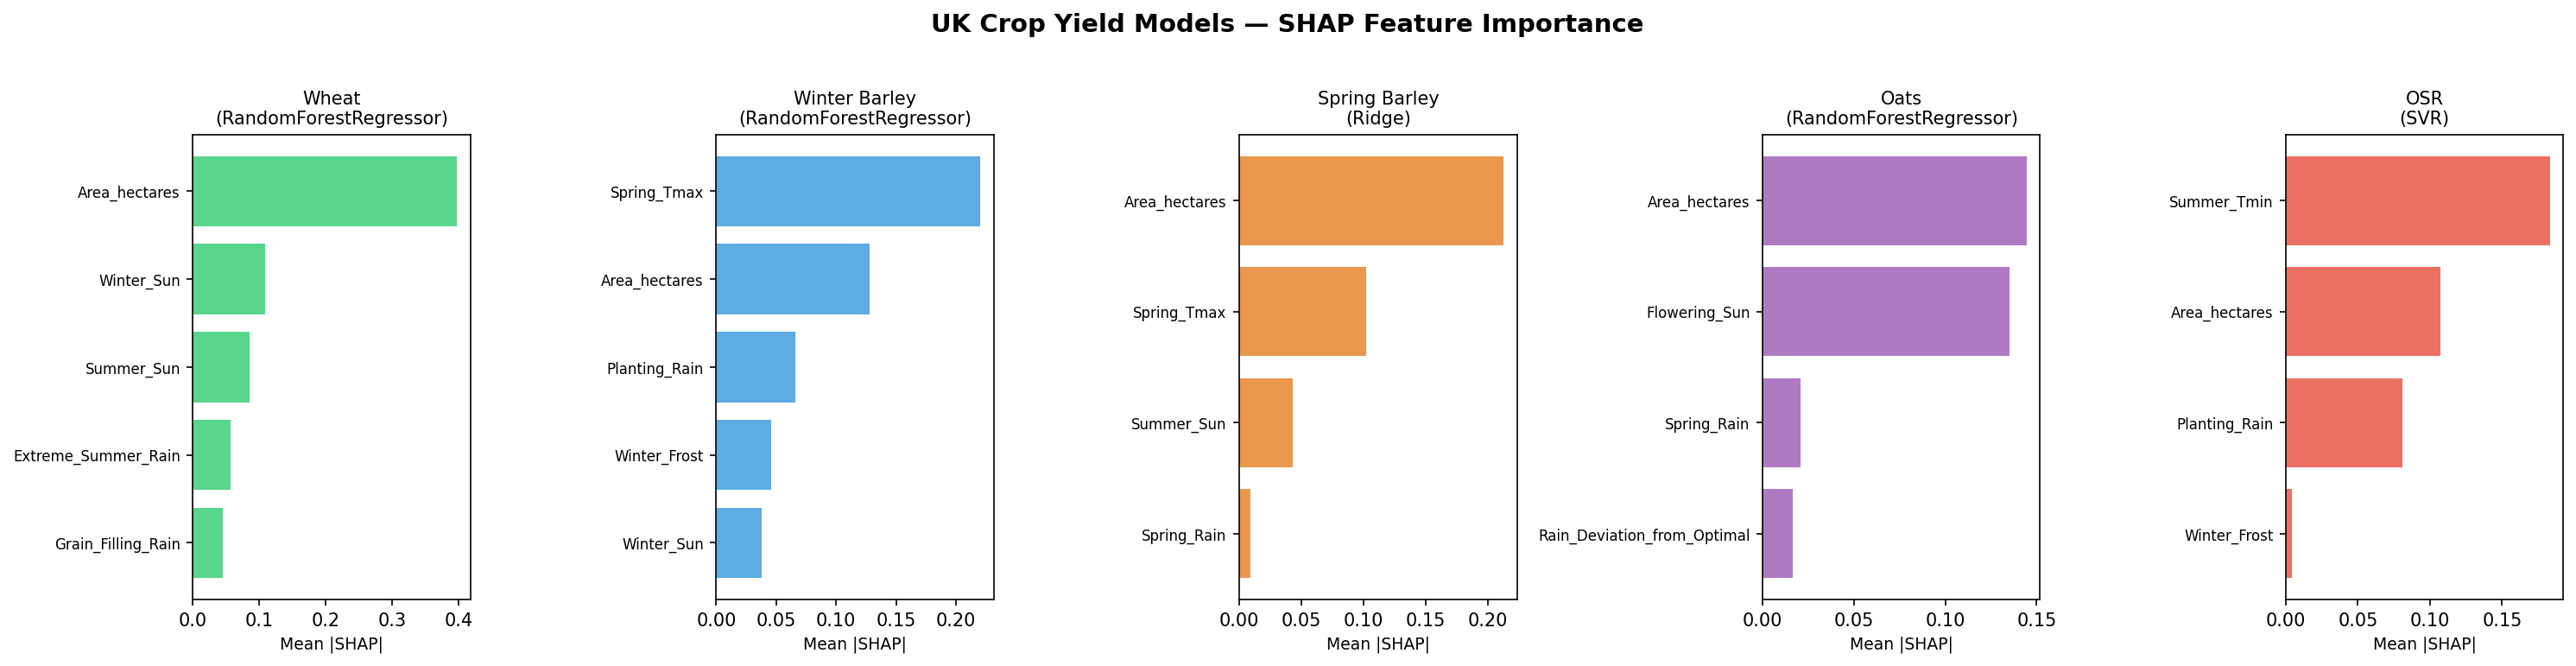
\includegraphics[width=0.95\textwidth]{shap_uk_panel.png}
\caption{SHAP feature importance for UK-only models across all five crops. Each bar shows the mean absolute SHAP value---the average impact of that feature on model predictions. Crop-specific weather sensitivities are clearly visible: wheat responds to winter sunshine, spring barley to spring rainfall.}
\label{fig:shap_uk}
\end{figure}

\begin{figure}[H]
\centering
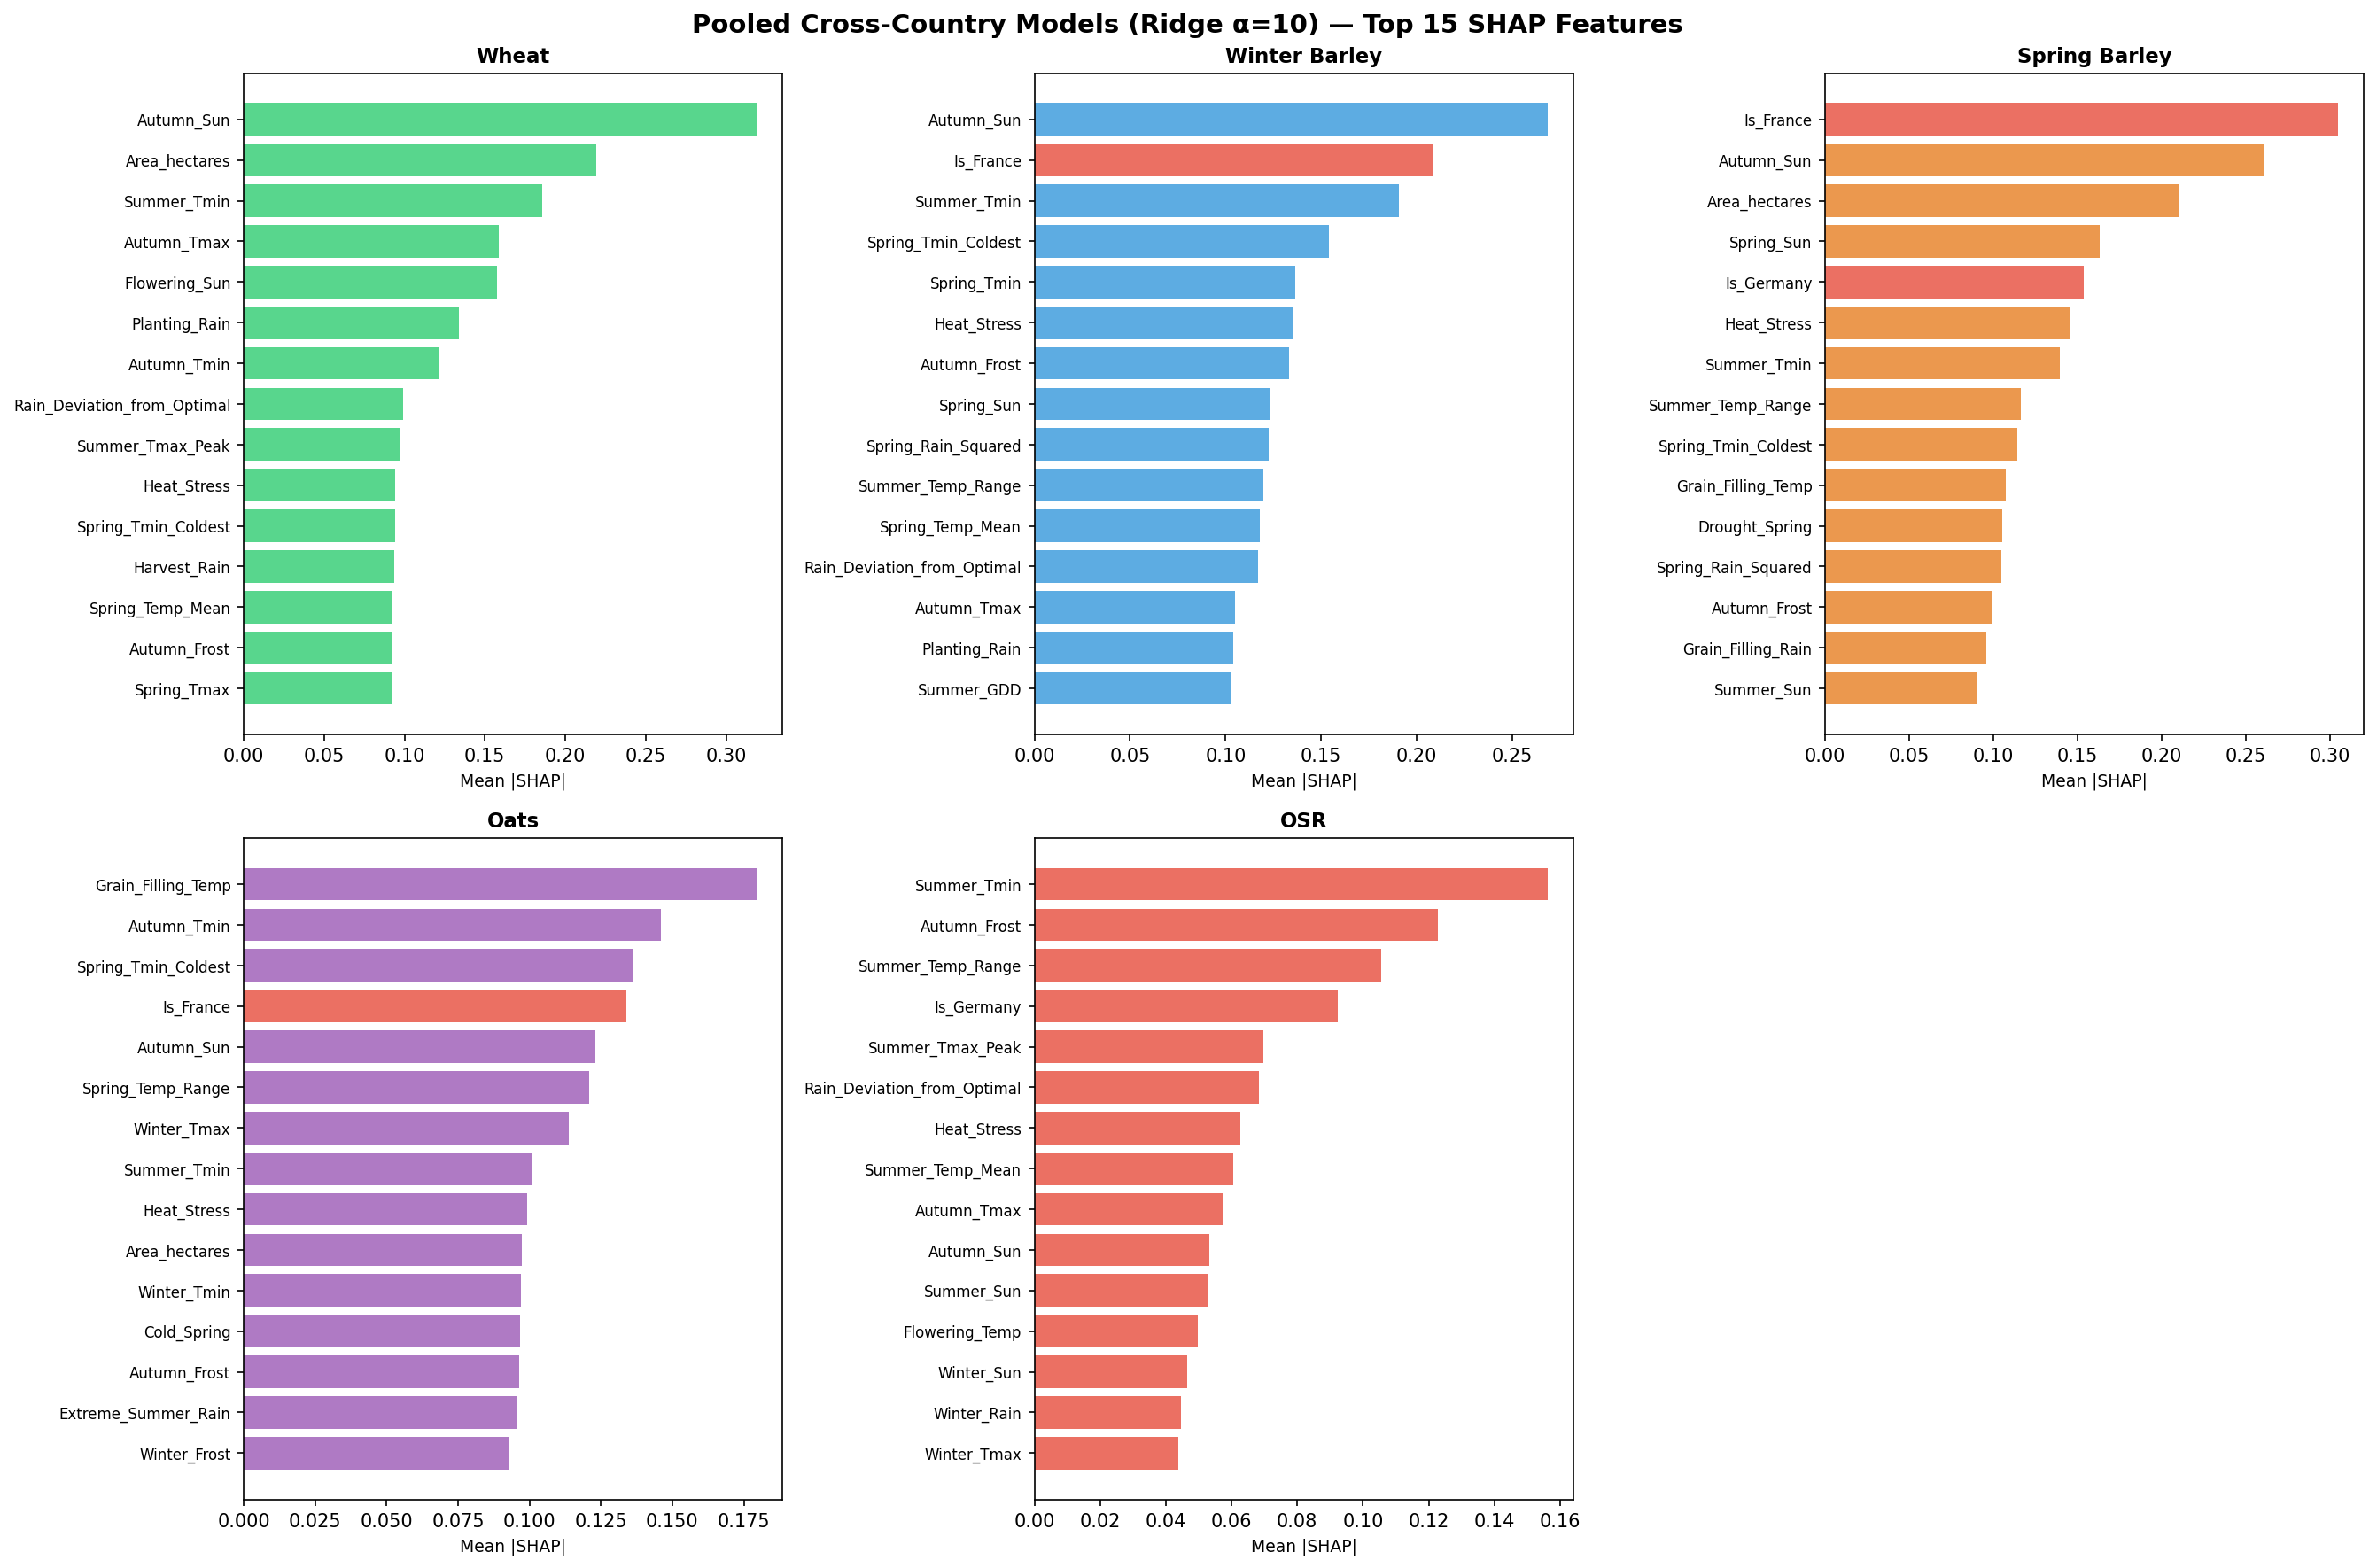
\includegraphics[width=0.95\textwidth]{shap_pooled_top_features.png}
\caption{Top 15 features by SHAP importance in the pooled cross-country model. Country indicators (Is\_France, Is\_Germany) appear with non-trivial importance, confirming that country-level differences are captured by the model alongside weather effects.}
\label{fig:shap_pooled}
\end{figure}

\begin{figure}[H]
\centering
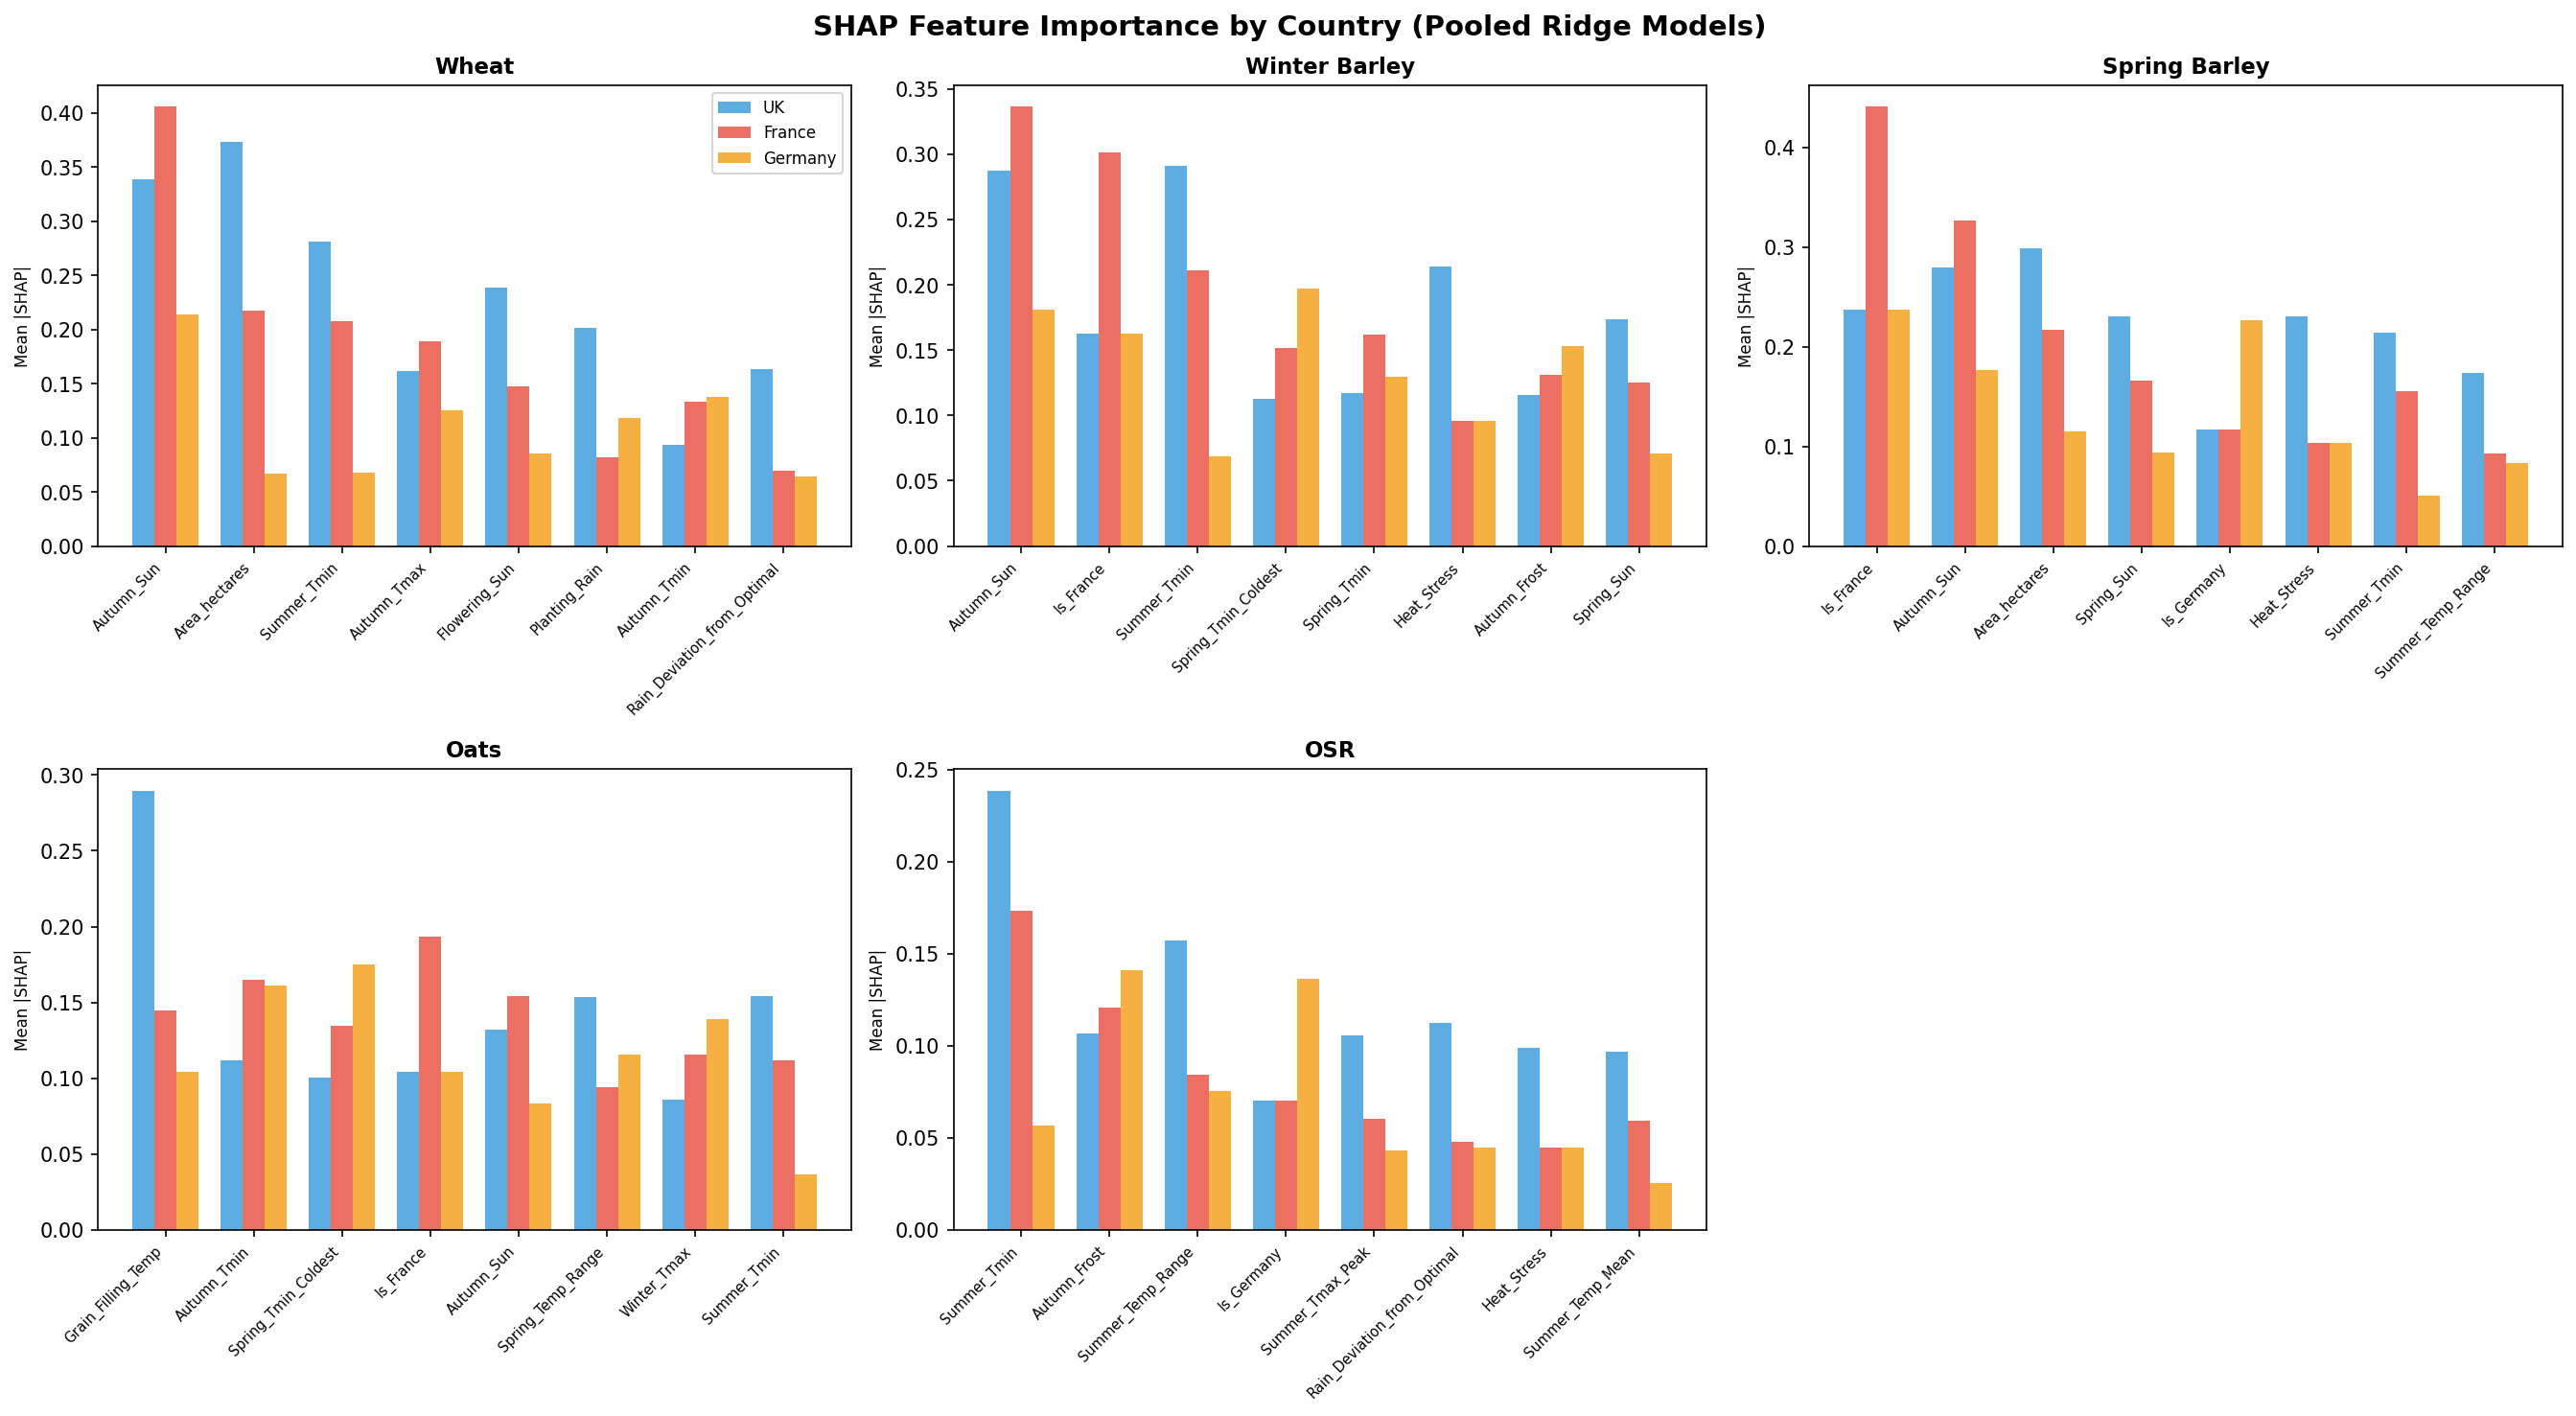
\includegraphics[width=0.95\textwidth]{shap_country_comparison.png}
\caption{SHAP importance comparison by country. Some features matter universally (Summer Tmax affects all countries), while others are country-specific (Winter Sun matters most for UK, reflecting the maritime climate's characteristic low winter light).}
\label{fig:shap_country}
\end{figure}

\begin{figure}[H]
\centering
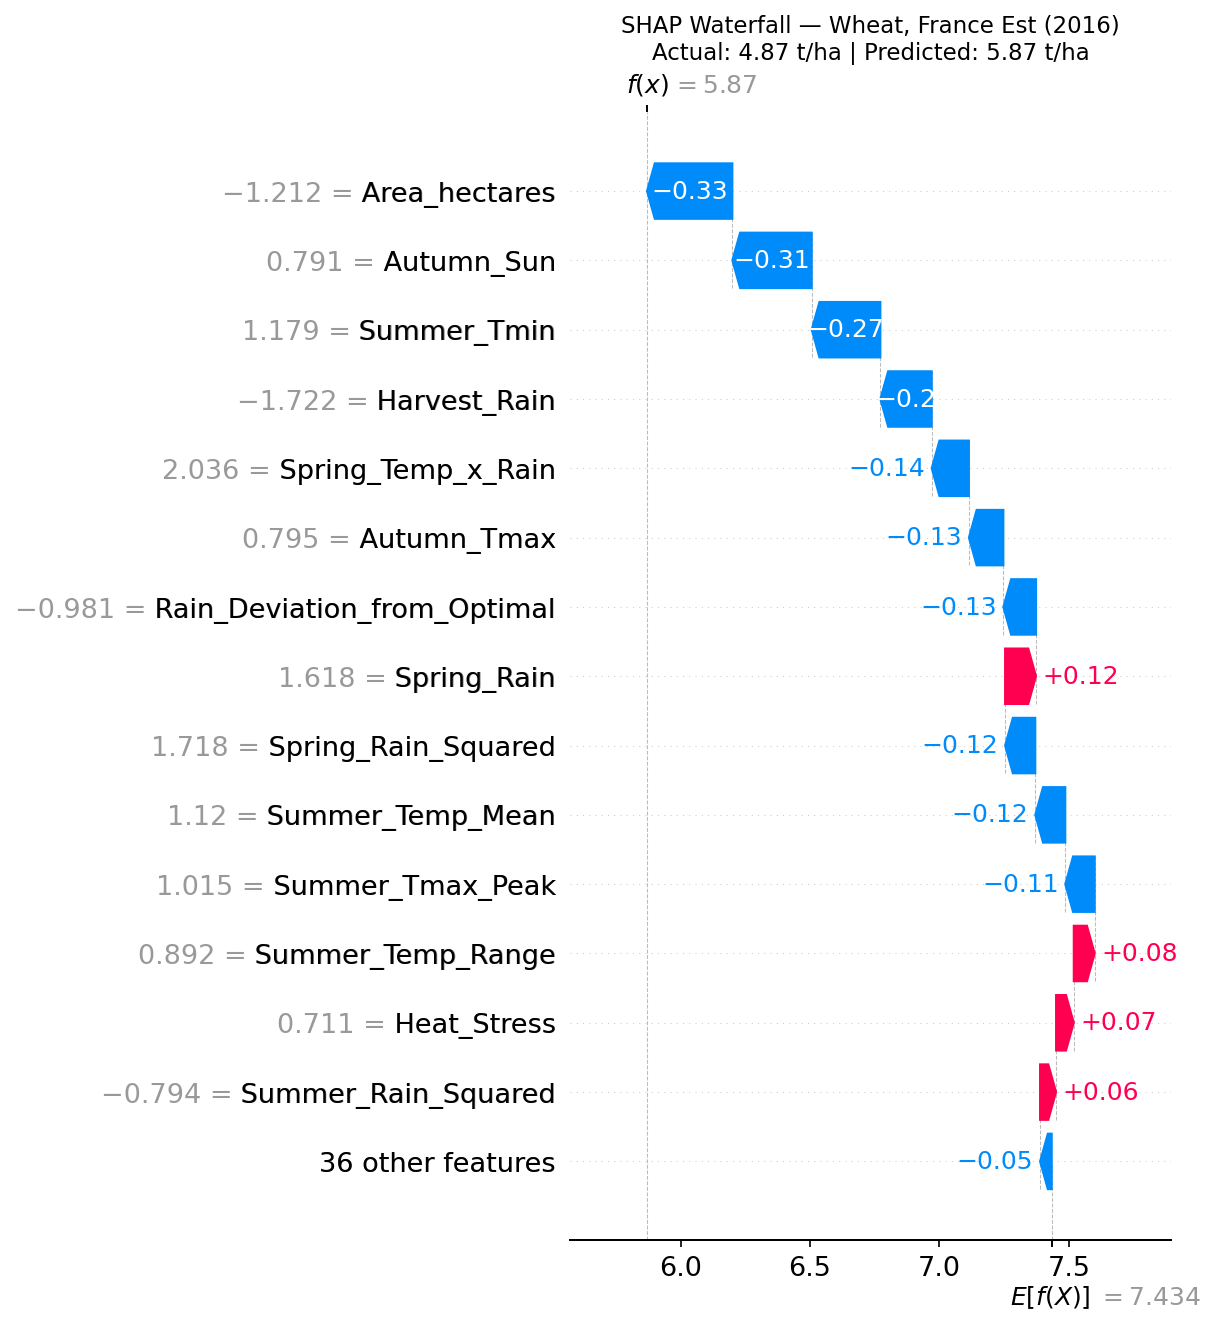
\includegraphics[width=0.95\textwidth]{shap_waterfall_example.png}
\caption{SHAP waterfall plot for a single observation (2018 drought year), showing how each feature pushes the prediction above or below the base value. This demonstrates the model's interpretability---individual predictions can be explained in terms of specific weather conditions.}
\label{fig:shap_waterfall}
\end{figure}

% --------------------------------------------------
\section{Deployed Flask Application}
% --------------------------------------------------

The final pooled anomaly models were deployed in a Flask web application with the following production performance:

\begin{table}[H]
\centering
\caption{Production model performance in the Flask application (LOOCV \rsq{}). These models use pooled France+UK anomaly data with Ridge regression. Of the 47~engineered weather features, 45 are retained after removing features with near-zero variance in the pooled dataset.}
\label{tab:flask_models}
\begin{tabular}{lcccc}
\toprule
\textbf{Crop} & \textbf{Algorithm} & \textbf{$\alpha$} & \textbf{LOOCV \rsq{}} & \textbf{Base yield (\tha{})} \\
\midrule
Wheat & Ridge & 1 & 0.682 & 7.65 \\
Winter Barley & Ridge & 1 & 0.624 & 6.66 \\
Spring Barley & Ridge & 100 & 0.760 & 5.22 \\
Oats & Ridge & 10 & 0.492 & 5.57 \\
OSR & Ridge & 1 & 0.443 & 3.40 \\
\bottomrule
\end{tabular}
\end{table}

% Placeholder for Flask app screenshot — you can add one later
% \begin{figure}[H]
% \centering
% \includegraphics[width=0.85\textwidth]{flask_app_screenshot.png}
% \caption{Flask web application prediction interface showing crop-specific weather feature sliders and yield prediction output.}
% \label{fig:flask_app}
% \end{figure}


% ============================================================================
% CHAPTER 5: DISCUSSION
% ============================================================================
\chapter{Discussion}

\section{Key Findings}

This project produced three main findings:

\textbf{Finding 1: Detrending and anomalisation enable effective cross-country data pooling.} The combination of yield detrending (removing technology trends) and weather z-score standardisation (removing climate baselines) transforms the cross-country pooling problem from one that fails catastrophically (\rsq{} = $-32$) to one that produces strong results (\rsq{} up to 0.76). This is not a novel statistical technique---both detrending \citep{moore2015} and standardisation are well-established---but their systematic application as a data augmentation strategy for crop yield prediction addresses a practical gap identified by \citet{corcoran2023}.

\textbf{Finding 2: Weather--yield response curves are transferable between countries.} The rescaled transfer results (Section~\ref{sec:anomaly_results}) demonstrate that a model trained exclusively on French anomaly data captures weather--yield relationships that are valid for the UK. The raw correlations between French model predictions and UK actual anomalies ($r = 0.41$--$0.82$) confirm that the \emph{direction} of weather effects is shared. This is consistent with the finding that wheat and barley share fundamental physiological responses to temperature and rainfall stress regardless of cultivar or location \citep{challinor2014}. The fact that a simple 2-parameter linear calibration rescues the predictions from catastrophic negatives (worst case \rsq{} $\approx -49$) to positive values across all five crops (best \rsq{} $= 0.65$ for spring barley) shows that the main difference between countries is one of magnitude, not shape.

\textbf{Finding 3: Static pooling is optimal; adaptive source selection does not help.} The z-score anomalisation already removes the climate baseline differences that would make dynamic country selection valuable. Once all countries' weather features express relative abnormality, there is no ``hot year $\to$ French data is more relevant'' effect left to exploit. In other words, the anomalisation step (Finding~1) does the work that scenario-adaptive source selection would otherwise need to do, which is why no adaptive scheme could improve on static pooling. This is a valuable negative result that confirms the anomalisation is doing its job comprehensively.

\section{Why Anomaly Transfer Works}

The success of the anomaly approach can be understood through the decomposition it imposes:

\begin{equation}
    \underbrace{Y_{it}}_{\text{actual yield}} = \underbrace{\hat{Y}_{\text{trend},i}(t)}_{\text{technology (country-specific)}} + \underbrace{f(\mathbf{z}_{it})}_{\text{weather response (transferable)}} + \varepsilon_{it}
\end{equation}

This decomposition succeeds because:

\begin{enumerate}
    \item \textbf{Technology trends are country-specific but smooth and predictable.} A linear trend captures most of the long-term yield variation due to improved varieties and practices. This component needs only a few data points per region to estimate---no cross-country transfer is needed.

    \item \textbf{Weather responses are noisy but physiologically universal.} How wheat responds to drought is governed by plant physiology, not by which country the field is in. By expressing weather as z-scores, we compare ``how stressed is this crop relative to its local norm?'' rather than ``what is the absolute temperature?''

    \item \textbf{The error term captures country-specific factors} (soil quality, pest pressure, management practices) that neither the trend nor the weather response can model. These factors add noise but do not bias the weather coefficients if they are uncorrelated with weather z-scores---a reasonable assumption.
\end{enumerate}

This explanation is consistent with \citet{evans2025}'s finding that space-for-time substitution works better for \emph{relative} impacts than for absolute predictions. By transferring response \emph{shapes} rather than \emph{levels}, we avoid the main pitfall they identify.

\section{Practical Implications}

\begin{enumerate}
    \item \textbf{For UK agriculture:} The pooled anomaly models provide substantially better yield forecasts than UK-only models, particularly for underserved crops (oats, spring barley, OSR). The deployed Flask application demonstrates that these models can be used for practical scenario analysis.

    \item \textbf{For data-scarce regions:} The methodology is applicable to any region with limited yield data but access to climatically similar neighbours. The key requirements are: (a)~yield data from at least one partner country growing the same crops, (b)~gridded weather data (E-OBS covers all of Europe), and (c)~detrending and z-scoring of both yield and weather data.

    \item \textbf{For climate adaptation:} The transferability of weather response curves, combined with \citet{ceglar2019}'s finding that agro-climate zones are migrating northward, suggests that current French weather--yield patterns may inform UK agricultural planning for a warming climate. This claim is qualified, however, by the non-stationarity concern raised in Limitation~5: the approach assumes the \emph{shape} of the response curve remains stable as the local climate baseline shifts, which is plausible but not guaranteed.
\end{enumerate}

\section{Limitations}

\begin{enumerate}
    \item \textbf{Small absolute sample sizes:} Even after pooling, the largest dataset (France+UK) has on the order of 150--200 observations per crop. This limits the complexity of learnable patterns and makes LOOCV results sensitive to individual outlier years.

    \item \textbf{Linear assumptions:} Ridge regression assumes linear relationships between weather z-scores and yield anomalies. Non-linear effects (e.g., threshold responses to extreme heat) may be underestimated. However, non-linear models (Random Forest, SVR) performed worse in our experiments, likely due to overfitting on small samples.

    \item \textbf{Spatial aggregation:} UK data is aggregated to four broad regions, masking within-region variability. England's East Anglia (dry, continental-influenced) and South West (wet, maritime) have very different weather--yield dynamics that are averaged together.

    \item \textbf{Missing non-weather factors:} Pest pressure (particularly for OSR), soil quality, and management practices are not modelled. OSR's modest \rsq{} (0.585 at best in the long-history transfer experiments, 0.443 in the deployed Flask model) likely reflects the dominance of cabbage stem flea beetle impacts over weather effects.

    \item \textbf{Temporal limitation:} The common evaluation period (2004--2016) is only 13~years, and LOOCV results may not generalise to future decades if climate change alters the weather--yield relationships themselves (non-stationarity).

    \item \textbf{Detrending assumes a stable trend:} Linear detrending assumes technology improvements are constant over time. If yield growth plateaus (as some evidence suggests for European wheat \citep{moore2015}), the linear trend may overestimate recent expected yields, biasing the anomalies.
\end{enumerate}


% ============================================================================
% CHAPTER 6: CONCLUSIONS AND FUTURE WORK
% ============================================================================
\chapter{Conclusions and Future Work}

\section{Conclusions}

This project developed and evaluated machine learning models for UK crop yield prediction, addressing the fundamental challenge of data scarcity through cross-country data augmentation. The main contributions are:

\begin{enumerate}
    \item \textbf{UK-only baseline models} for five crops using 47~engineered weather features, achieving \rsq{} = 0.15--0.50 and identifying crop-specific weather sensitivities (winter sunshine for wheat, spring rainfall for barley, pest dominance for OSR).

    \item \textbf{A systematic evaluation of cross-country data pooling}, demonstrating that na\"{\i}ve pooling and classical domain adaptation methods (mixed effects, CORAL, bias correction) improve pooled prediction but fail at direct transfer.

    \item \textbf{A detrended anomaly transfer methodology} that combines yield detrending with weather z-score standardisation, enabling meaningful cross-country data combination and improving LOOCV \rsq{} from 0.22 to 0.76 (spring barley), 0.28 to 0.70 (wheat), and $-0.46$ to 0.48 (oats).

    \item \textbf{Evidence of cross-country transferability}: weather--yield response curves learned from French data alone can predict UK yield anomalies with positive \rsq{} (0.14--0.65) after minimal calibration, confirming that the physiological responses of crops to weather stress are shared across countries.

    \item \textbf{A negative result} showing that scenario-adaptive source country selection offers no improvement over static pooling, confirming that z-score anomalisation comprehensively addresses climate baseline differences.

    \item \textbf{A deployed Flask web application} integrating the pooled anomaly models for interactive crop yield prediction.
\end{enumerate}

\section{Future Work}

\begin{enumerate}
    \item \textbf{Prediction intervals:} Currently the models output point predictions. Adding uncertainty quantification (e.g., conformal prediction, bootstrap intervals) would make the predictions more practically useful.

    \item \textbf{Temporal out-of-sample validation:} Training on 2004--2018 and testing on 2019--2024 would provide a more realistic assessment of forecast skill than LOOCV.

    \item \textbf{Non-linear anomaly models:} Gradient-boosted trees or neural networks applied to the anomaly data may capture threshold effects (e.g., heat stress above 30\degrees{}) that Ridge regression misses, provided the sample size is sufficient.

    \item \textbf{Higher spatial resolution:} Replacing the four UK regions with county-level or grid-cell-level data would increase sample size and capture within-region heterogeneity.

    \item \textbf{Climate change projections:} Using UKCP18 climate projections as inputs to the anomaly model could provide forward-looking yield scenarios under different warming pathways.

    \item \textbf{Extension to more countries:} \citet{ronchetti2024}'s harmonised EU dataset covers 27~countries; extending the pipeline beyond 7~countries could further improve the anomaly models, though our results suggest diminishing returns.
\end{enumerate}


% ============================================================================
% REFERENCES
% ============================================================================
\bibliographystyle{plainnat}

\begin{thebibliography}{99}

\bibitem[AHDB(2023a)]{ahdb2023a}
AHDB (2023a).
\newblock \emph{UK Wheat Production Statistics}.
\newblock Agriculture and Horticulture Development Board.

\bibitem[AHDB(2023c)]{ahdb2023c}
AHDB (2023c).
\newblock \emph{Oilseed Rape Guide}.
\newblock Agriculture and Horticulture Development Board.

\bibitem[Battisti \& Naylor(2009)]{battisti2009}
Battisti, D.S. and Naylor, R.L. (2009).
\newblock Historical warnings of future food insecurity with unprecedented seasonal heat.
\newblock \emph{Science}, 323(5911), 240--244.

\bibitem[Ceglar et~al.(2019)]{ceglar2019}
Ceglar, A., Zampieri, M., Toreti, A. and Dentener, F. (2019).
\newblock Observed northward migration of agro-climate zones in Europe will further accelerate under climate change.
\newblock \emph{Earth's Future}, 7(9), 1088--1101.

\bibitem[Challinor et~al.(2014)]{challinor2014}
Challinor, A.J., Watson, J., Lobell, D.B., Howden, S.M., Smith, D.R. and Chhetri, N. (2014).
\newblock A meta-analysis of crop yield under climate change and adaptation.
\newblock \emph{Nature Climate Change}, 4(4), 287--291.

\bibitem[Chlingaryan et~al.(2018)]{chlingaryan2018}
Chlingaryan, A., Sukkarieh, S. and Whelan, B. (2018).
\newblock Machine learning approaches for crop yield prediction and nitrogen status estimation in precision agriculture: A review.
\newblock \emph{Computers and Electronics in Agriculture}, 151, 61--69.

\bibitem[Corcoran et~al.(2023)]{corcoran2023}
Corcoran, E., Afshar, M., Curceac, S., Lashkari, A., Raza, M.M., Ahnert, S., Mead, A. and Morris, R. (2023).
\newblock Current data and modeling bottlenecks for predicting crop yields in the United Kingdom.
\newblock \emph{Frontiers in Sustainable Food Systems}, 7, 1023169.

\bibitem[Cornes et~al.(2018)]{cornes2018}
Cornes, R.C., van~der Schrier, G., van~den Besselaar, E.J.M. and Jones, P.D. (2018).
\newblock An ensemble version of the E-OBS temperature and precipitation data sets.
\newblock \emph{Journal of Geophysical Research: Atmospheres}, 123(17), 9391--9409.

\bibitem[DEFRA(2012)]{defra2012}
DEFRA (2012).
\newblock \emph{Farming Statistics: Final Crop Areas, Yields, Livestock Populations and Agricultural Workforce}.
\newblock Department for Environment, Food and Rural Affairs.

\bibitem[DEFRA(2023)]{defra2023}
DEFRA (2023).
\newblock \emph{Agriculture in the United Kingdom 2022}.
\newblock Department for Environment, Food and Rural Affairs.

\bibitem[DEFRA(2024)]{defra2024}
DEFRA (2024).
\newblock \emph{Cereal and Oilseed Rape Production in the United Kingdom}.
\newblock Department for Environment, Food and Rural Affairs.

\bibitem[Dinh \& Aires(2022)]{dinh2022}
Dinh, T.L.A. and Aires, F. (2022).
\newblock Nested leave-two-out cross-validation for the optimal crop yield model selection.
\newblock \emph{Geoscientific Model Development}, 15, 3519--3535.

\bibitem[Evans et~al.(2025)]{evans2025}
Evans, M.E.K., Adler, P.B., Angert, A.L. et~al. (2025).
\newblock Reconsidering space-for-time substitution in climate change ecology.
\newblock \emph{Nature Climate Change}, 15(8), 809--812.

\bibitem[Gammans et~al.(2017)]{gammans2017}
Gammans, M., Merel, P. and Ortiz-Bobea, A. (2017).
\newblock Negative impacts of climate change on cereal yields: Statistical evidence from France.
\newblock \emph{Environmental Research Letters}, 12(5), 054007.

\bibitem[IPCC(2021)]{ipcc2021}
IPCC (2021).
\newblock \emph{Climate Change 2021: The Physical Science Basis}.
\newblock Contribution of Working Group~I to the Sixth Assessment Report.

\bibitem[Jeong et~al.(2016)]{jeong2016}
Jeong, J.H., Resop, J.P., Mueller, N.D. et~al. (2016).
\newblock Random forests for global and regional crop yield predictions.
\newblock \emph{PLoS ONE}, 11(6), e0156571.

\bibitem[Lobell \& Burke(2010)]{lobell2010}
Lobell, D.B. and Burke, M.B. (2010).
\newblock On the use of statistical models to predict crop yield responses to climate change.
\newblock \emph{Agricultural and Forest Meteorology}, 150(11), 1443--1452.

\bibitem[Met Office(2024)]{metoffice2024}
Met Office (2024).
\newblock \emph{UK and Regional Climate Series}.
\newblock Available at: \url{https://www.metoffice.gov.uk/research/climate/maps-and-data/uk-and-regional-series}.

\bibitem[Moore \& Lobell(2015)]{moore2015}
Moore, F.C. and Lobell, D.B. (2015).
\newblock The fingerprint of climate trends on European crop yields.
\newblock \emph{PNAS}, 112(9), 2670--2675.

\bibitem[Pan \& Yang(2010)]{pan2010}
Pan, S.J. and Yang, Q. (2010).
\newblock A survey on transfer learning.
\newblock \emph{IEEE Transactions on Knowledge and Data Engineering}, 22(10), 1345--1359.

\bibitem[Paudel et~al.(2021)]{paudel2021}
Paudel, D., Boogaard, H., de~Wit, A., Janssen, S., Osinga, S., Pylianidis, C. and Athanasiadis, I.N. (2021).
\newblock Machine learning for large-scale crop yield forecasting.
\newblock \emph{Agricultural Systems}, 187, 103016.

\bibitem[Pugh et~al.(2016)]{pugh2016}
Pugh, T.A.M., M\"{u}ller, C., Elliott, J. et~al. (2016).
\newblock Climate analogues suggest limited potential for intensification of production on current croplands under climate change.
\newblock \emph{Nature Communications}, 7, 12608.

\bibitem[Riedesel et~al.(2024)]{riedesel2024}
Riedesel, L., Moller, M., Piepho, H.-P., Rentel, D., Lichthardt, C., Golla, B., Kautz, T. and Feike, T. (2024).
\newblock Site conditions determine heat and drought induced yield losses in wheat and rye in Germany.
\newblock \emph{Environmental Research Letters}, 19, 034024.

\bibitem[Ronchetti et~al.(2024)]{ronchetti2024}
Ronchetti, G., Nisini~Scacchiafichi, L., Seguini, L., Cerrani, I. and van~der~Velde, M. (2024).
\newblock Harmonized European Union subnational crop statistics can reveal climate impacts and crop cultivation shifts.
\newblock \emph{Earth System Science Data}, 16, 1623--1649.

\bibitem[Schauberger et~al.(2018)]{schauberger2018}
Schauberger, B., Ben-Ari, T., Makowski, D., Kato, T., Kato, H. and Ciais, P. (2018).
\newblock Yield trends, variability and stagnation analysis of major crops in France over more than a century.
\newblock \emph{Scientific Reports}, 8, 16865.

\bibitem[United Nations(2019)]{un2019}
United Nations (2019).
\newblock \emph{World Population Prospects 2019}.
\newblock Department of Economic and Social Affairs.

\bibitem[van~Klompenburg et~al.(2020)]{vanklompenburg2020}
van~Klompenburg, T., Kassahun, A. and Catal, C. (2020).
\newblock Crop yield prediction using machine learning: A systematic literature review.
\newblock \emph{Computers and Electronics in Agriculture}, 177, 105709.

\bibitem[Zhao et~al.(2017)]{zhao2017}
Zhao, C., Liu, B., Piao, S. et~al. (2017).
\newblock Temperature increase reduces global yields of major crops in four independent estimates.
\newblock \emph{Proceedings of the National Academy of Sciences}, 114(35), 9326--9331.

\bibitem[Zheng et~al.(2012)]{zheng2012}
Zheng, B., Chenu, K., Dreccer, M.F. and Chapman, S.C. (2012).
\newblock Breeding for the future: what are the potential impacts of future frost and heat events on sowing and flowering time requirements for Australian bread wheat (\emph{Triticum aestivum}) varieties?
\newblock \emph{Global Change Biology}, 18(9), 2899--2914.

\bibitem[Zhu et~al.(2021)]{zhu2021}
Zhu, P., Abramoff, R., Makowski, D. and Ciais, P. (2021).
\newblock Uncovering the past and future climate drivers of wheat yield shocks in Europe with machine learning.
\newblock \emph{Earth's Future}, 9(5), e2020EF001815.

\end{thebibliography}


% ============================================================================
% APPENDICES
% ============================================================================
\appendix

\chapter{Complete Weather Feature List}

\begin{longtable}{lll}
\caption{All 47 engineered weather features} \label{tab:all_features} \\
\toprule
\textbf{Category} & \textbf{Feature} & \textbf{Description} \\
\midrule
\endfirsthead
\toprule
\textbf{Category} & \textbf{Feature} & \textbf{Description} \\
\midrule
\endhead
\bottomrule
\endfoot
Temperature & Winter\_Tmax & Mean daily max temp, Dec--Feb \\
& Spring\_Tmax & Mean daily max temp, Mar--May \\
& Summer\_Tmax & Mean daily max temp, Jun--Aug \\
& Autumn\_Tmax & Mean daily max temp, Sep--Nov \\
& Winter\_Tmin & Mean daily min temp, Dec--Feb \\
& Spring\_Tmin & Mean daily min temp, Mar--May \\
& Summer\_Tmin & Mean daily min temp, Jun--Aug \\
& Autumn\_Tmin & Mean daily min temp, Sep--Nov \\
& Spring\_Temp\_Mean & Mean temp, Mar--May \\
& Summer\_Temp\_Mean & Mean temp, Jun--Aug \\
& Flowering\_Temp & Mean temp, May--Jun \\
& Grain\_Filling\_Temp & Mean temp, Jul--Aug \\
& Summer\_Tmax\_Peak & Max of monthly Tmax, Jun--Aug \\
& Spring\_Tmin\_Coldest & Min of monthly Tmin, Mar--May \\
& Spring\_Temp\_Range & Tmax $-$ Tmin range, Mar--May \\
& Summer\_Temp\_Range & Tmax $-$ Tmin range, Jun--Aug \\
& Spring\_GDD & Growing degree days, Mar--May \\
& Summer\_GDD & Growing degree days, Jun--Aug \\
\midrule
Rainfall & Winter\_Rain & Total rainfall, Dec--Feb (mm) \\
& Spring\_Rain & Total rainfall, Mar--May (mm) \\
& Summer\_Rain & Total rainfall, Jun--Aug (mm) \\
& Autumn\_Rain & Total rainfall, Sep--Nov (mm) \\
& Planting\_Rain & Total rainfall, Sep--Oct (mm) \\
& Grain\_Filling\_Rain & Total rainfall, Jul--Aug (mm) \\
& Harvest\_Rain & Total rainfall, Aug (mm) \\
& Annual\_Rain & Total annual rainfall (mm) \\
& Rain\_Deviation\_from\_Optimal & $|$Rain $-$ optimal$|$ \\
& Spring\_Rain\_Squared & Spring rainfall squared \\
& Summer\_Rain\_Squared & Summer rainfall squared \\
\midrule
Sunshine & Winter\_Sun & Total sunshine hours, Dec--Feb \\
& Spring\_Sun & Total sunshine hours, Mar--May \\
& Summer\_Sun & Total sunshine hours, Jun--Aug \\
& Autumn\_Sun & Total sunshine hours, Sep--Nov \\
& Grain\_Filling\_Sun & Sunshine hours, Jul--Aug \\
& Flowering\_Sun & Sunshine hours, May--Jun \\
& Summer\_Sun\_per\_Rain & Summer sunshine / rainfall ratio \\
\midrule
Frost & Winter\_Frost & Frost days ($<$0\degrees{}), Dec--Feb \\
& Spring\_Frost & Frost days ($<$0\degrees{}), Mar--May \\
& Autumn\_Frost & Frost days ($<$0\degrees{}), Sep--Nov \\
& Late\_Spring\_Frost & Frost days, Apr--May \\
\midrule
Interactions & Spring\_Temp\_x\_Rain & Spring temp $\times$ rainfall \\
& Summer\_Temp\_x\_Rain & Summer temp $\times$ rainfall \\
& Summer\_Temp\_x\_Sun & Summer temp $\times$ sunshine \\
& Heat\_Stress & Binary: Tmax $>$ 30\degrees{} \\
& Cold\_Spring & Binary: Spring Tmin $<$ 2\degrees{} \\
& Extreme\_Summer\_Rain & Binary: Summer rain $>$ 300\,mm \\
& Drought\_Spring & Binary: Spring rain $<$ 100\,mm \\
\end{longtable}


\chapter{Eurostat Crop Codes}

\begin{table}[H]
\centering
\caption{Eurostat crop codes used for data collection}
\begin{tabular}{lll}
\toprule
\textbf{Code} & \textbf{Crop} & \textbf{Our label} \\
\midrule
C1110 & Soft wheat and spelt & Wheat \\
C1310 & Winter barley & Winter Barley \\
C1320 & Spring barley & Spring Barley \\
C1410 & Oats & Oats \\
I1110 & Rapeseed and turnip rapeseed & OSR \\
\bottomrule
\end{tabular}
\end{table}


\end{document}
